\chapter{Motivación y Antecedentes}
\section{Crecimiento de la red}
El gran crecimiento en la cantidad de sistemas tecnológicos interconectados vía Internet en el mundo en los últimos 30 años es algo que no ha dejado indiferente a nadie\footnote{\url{http://www.internetworldstats.com/emarketing.htm}}. Para entender este fenómeno distintos organismos internacionales se dedican periódicamente a realizar estimaciones de dicha cifra. Un caso muy popular de esta labor es el contador global de conexiones móviles a Internet del \emph{GSMA Intelligence}\footnote{\url{https://gsmaintelligence.com/}} el cual recientemente ha estimado en más de 7 mil millones el número de dispositivos móviles con conexión a la red, superando por primera vez al total de la población mundial\footnote{\url{http://www.cnet.com/news/there-are-now-more-gadgets-on-earth-than-people/}}. Una premisa que coincide con el último informe \emph{The State Of Internet} de la corporación \emph{Akamai} \cite{report:akamai} donde se resume el estudio de las principales variaciones en capacidad de acceso, velocidades de acceso, tipos de ataques, etc. a Internet de que disponen distintos países del mundo. Éste estudio corroboró lo que ya ha sido tendencia en los últimos años: Tanto las velocidades de navegación, como el total de conexiones a Internet han aumentado generalizadamente en todo el planeta (Ver figura \ref{fig:akamai_stats}). Las proyecciones a futuro preservan ésta tendencia apostando a que tanto la cantidad de dispositivos como el número de accesos a Internet deberían seguir subiendo \cite{nota:2020}, ello producto de factores como la reducción de costos de producción y la minimización de la tecnología, además de distintas tendencias generadas a raíz del fenómeno de \emph{globalización} que --en gran medida-- nos ha forzado a participar de una sociedad más interconectada en todo el mundo. Olvidando un poco las interpretaciones o justificaciones para ésta situación, el hecho concreto es que existe una directa proporcionalidad entre el número de dispositivos y los requerimientos de accesos a la red, y hoy ambos están en su apogeo de crecimiento.

\begin{figure}[!h]
	\centering
	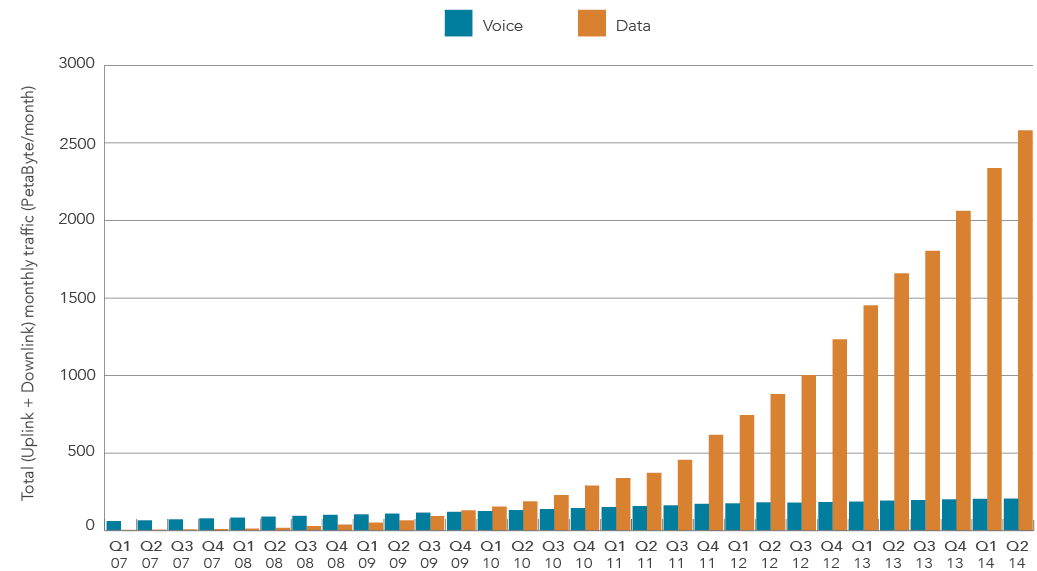
\includegraphics[scale=0.5]{imagenes/conexiones_moviles}
	\caption{Registros de la compañía \emph{Ericsson} ilustrando el crecimiento exponencial en el uso de datos de los dispositivos móviles. Parte del informe de \emph{Akamai} \cite{report:akamai}}
	\label{fig:akamai_stats}
\end{figure}

Más allá del número de dispositivos o la cantidad --o calidad-- del acceso a Internet, las distintas aplicaciones actuales han evolucionado sobre la base de protocolos y sistemas diseñados hace varias décadas, pero exigiendo siempre la mejor performance posible en pos de garantizar buenos tiempos de respuesta. Los protocolos más celebres de la llamada \emph{familia de protocolos de Internet} son TCP e IP. Sin embargo, son decenas los protocolos y mecanismos involucrados en las diferentes fases de comunicación entre computadoras y aplicaciones, que permiten en conjunto la operación de la red de redes como hoy la conocemos.

\section{El modelo OSI}
La capacidad de conectividad entre 2 distintos dispositivos es resultado del efecto combinado de varias capas de abstracción con responsabilidades divididas. Un diseño de operación que se ilustra en un modelo estándar vigente desde los años 80 es el impulsado por la \emph{Organización Internacional de Normalización} (ISO), mejor conocido como el modelo \textbf{OSI}\footnote{Por sus siglas en inglés \emph{Open System Interconnection}.}. En la práctica, la importancia de éste modelo radica en servir como una referencia técnica que ilustra los límites en las responsabilidades entre componentes que conforman una arquitectura de interconexión de sistemas.

El modelo OSI reconoce 7 capas de abstracción en el proceso de comunicación entre dispositivos (Ver figura \ref{fig:osi7capas}), cada una con obligaciones específicas, pero que combinadas soportan constructivamente un mecanismo de comunicación estándar para sistemas que por él se rijan. El acierto de éste enfoque está en permitir el desarrollo de soluciones modulares y especificas a cada una de las capas, sin interferir entre capas diferentes y manteniendo así la compatibilidad con aplicaciones que ya operen en capas distintas. Las 7 capas en cuestión se describen a continuación:

\begin{figure}[!h]
	\centering
	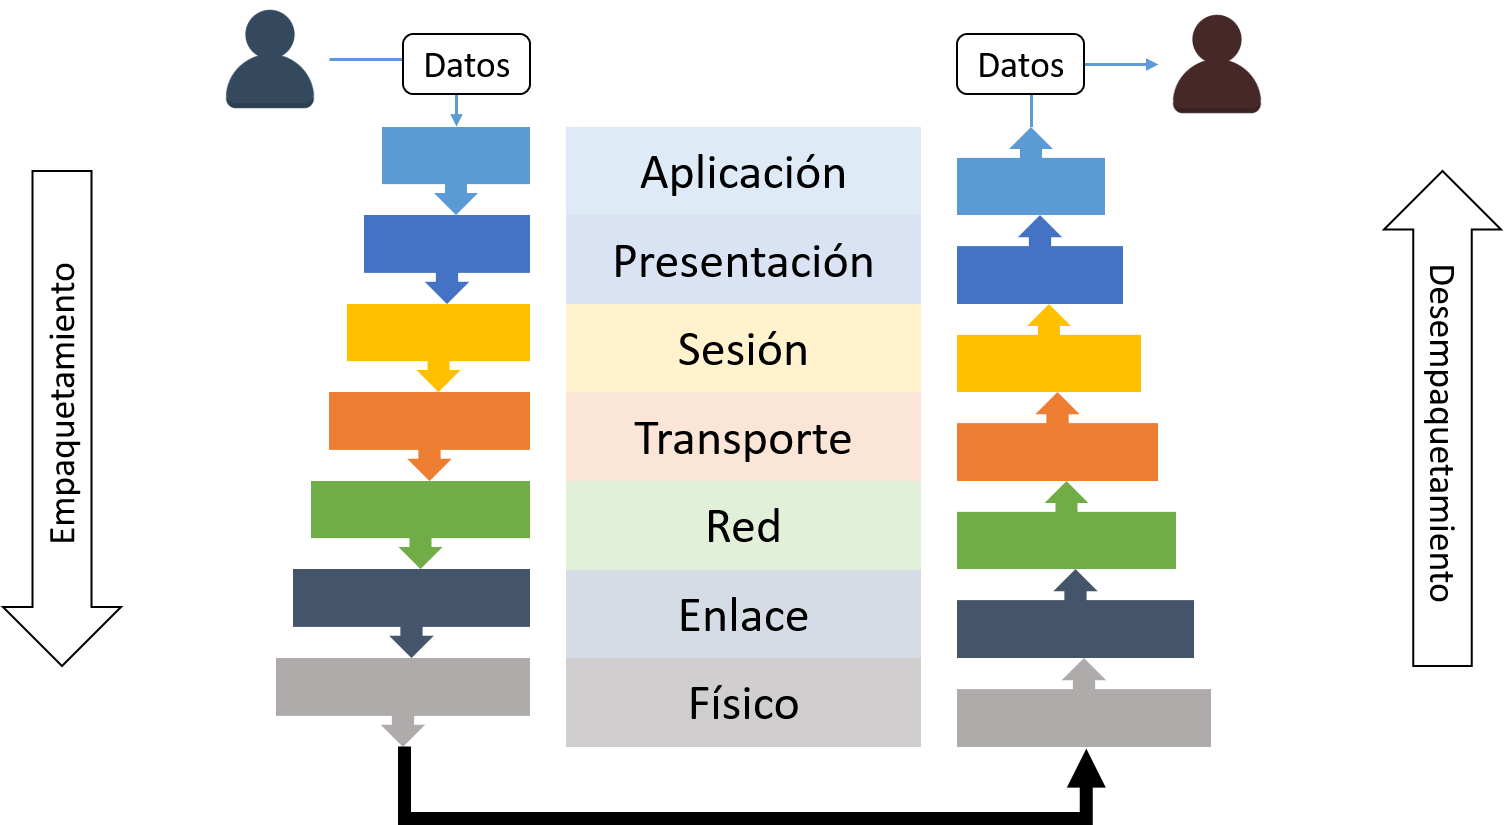
\includegraphics[scale=.45]{imagenes/OSI7Capas.png}
	\caption{Diagrama esquemático de las 7 capas del modelo OSI, ilustrando el proceso de encapsulamiento y desencapsulamiento de datos al ir agregando y removiendo encabezados de capa, según los procesos de empaquetamiento y desempaquetamiento, respectivamente.}
	\label{fig:osi7capas}
\end{figure}

\begin{description}
\item[Capa Física] La capa de nivel inferior en el modelo OSI es la capa física. Es ésta capa la responsible de la topología de la red y de la especificación de los medios materiales que consiguen la transmisión de la información, así como también es responsable de la generación real de la comunicación por medio del envío de la información. Es, en definitiva, la encargada del paso a canales físicos de la información a transmitir.

\item[Capa de Enlace] Es la segunda capa del modelo. Ella se encarga de proveer un mecanismo de direccionamiento físico en una máquina que permita el reconocimiento individual de la misma, proveiendo de un primer identificador a las máquinas en el modelo OSI dado por las direcciones físicas de los dispositivos (\emph{MAC}). Es responsable también de proveer mecanismos de corrección de errores en el proceso de transmisión de datos que pudiesen manifestarse por problemas de la capa física, haciendo dicha comunicación, desde éste punto, confiable.

\item[Capa de Red] Es la tercera capa del modelo OSI. Hace su debut en contextos de multiples equipos interconectados brindando mecanismos de identificación para proveer una capacidad de direccionamiento más amplia con respecto al disponible en las dos primeras capas (que sólo permitian la comunicación entre un par de máquinas, punto a punto). En éste nivel aparece uno de los protocolos más populares en Internet, el denominado protocolo IP que supone un mecanismo de identificación único para cada dispositivo en una red, provisto en base a una dirección homónima. Ésta capa establece la capacidad de ruteo en la comunicación como una responsabilidad de los nodos en una infraestructura en red, haciendo cada componente de la red alcanzable para cualquier otro integrante de la misma.

\item[Capa de Transporte] La cuarta capa del modelo, es la que provee de lleno la capacidad de transporte de datos. En éste nivel se incorporan los también celebres protocolos homónimos: TCP (orientado a la conexión) y UDP (orientado a la mensajería). Ésta capa es también responsible de brindar la capacidad de multiplexación a nivel de una máquina, permitiendo la generación de multiples conexiones desde el mismo dispositivo. Dicho mecanismo lo consigue al incorporar puertos numerados, que sirven como puntos lógicos de comunicación. De ésta manera, a partir de la capa de transporte se establece un paradigma base en el área de redes, en lo que a programación y esquematización de la misma corresponde: La construcción de conexiones \emph{IP:PUERTO}, que son la base del concepto de tuplas de direccionamiento en el proceso de transporte de datos.

\item[Capa de Sesión] Es la quinta capa del modelo OSI. Tal y como su nombre lo indica su función radica en ser la responsible de mantener un control de sesión en una conexión entre extremos, proveiendo mecanismos de corrección y reconexion en caso de interferencia de una operación entre máquinas. Es responsable de mantener el enlace de comunicación construido en base a las capas inferiores en un proceso de comunicación.

\item[Capa de Presentación] El sexto nivel en el modelo OSI es la capa de presentación, cuya responsabilidad comprende proveer el soporte para dar una correcta interpretación de los datos transmitidos, de manera de conseguir que los datos lleguen de manera reconocible al host de destino. A diferencia de las capas inferiores que se enfocan en los mecanismos de envío de la infromación, ésta capa guarda directa relación con la información transmitida y con su correcta interpretación final.

\item[Capa de Aplicación] Es la última -y de más alto nivel- capa de abstracción del modelo OSI. Es la responsible de proveer una interfaz simple a aplicaciones al acceso a mecanismos de comunicación en red. En otras palabras, es la responsible de proveer el servicio de comunicaciones a las distintas aplicaciones que tengan distintos requerimientos de comunicación.

\end{description}

A pesar de que el modelo OSI plantea responsabilidades delimitadas a cada capa de abstracción, la correspondencia de dicho estándar teórico en la práctica es una labor que queda supeditada a los programadores de sistemas operativos. Finalmente son ellos los que, en mayor o menor medida, hacen corresponder para con el modelo las implementaciones finales de los módulos de red de un sistema.


\section{Familia de Protocolos de Internet}
El conjunto de múltiples protocolos que facultan a los sistemas con mecanismos de interconexión comprende a varios cientos que se distribuyen entre las distintas capas del modelo OSI. A este conjunto se le denomina \emph{Familia de Protocolos de Internet}. Sin embargo, históricamente se le ha prestado especial atención a un subconjunto de ellos que son estructurales en la infraestructura predominante de Internet y que rigen la misma, hablamos del conjunto de protocolos \textbf{TCP/IP}.

La arquitectura de los protocolos TCP/IP sigue la inspiración del modelo OSI en las responsabilidades a soportar --a pesar de romper la estructura de capas del mismo-- combinando algunas responsabilidades de dicho modelo en funciones únicas y obviando otras. Un ejemplo de esto se puede apreciar en la tabla \ref{tabla:tcpiposi} que ilustra la correspondencia de los protocolos del conjunto TCP/IP con su atribución según el modelo OSI.

\begin{table}[h!]
\centering
\begin{tabular}{|c|p{4cm}|l|p{5cm}|}
\hline
\multicolumn{1}{|c|}{\textbf{\begin{tabular}[c]{@{}c@{}}Ref. OSI\\ Nº de capa\end{tabular}}} & \multicolumn{1}{c|}{\textbf{\begin{tabular}[c]{@{}c@{}}Equivalente \\ de capa OSI\end{tabular}}} & \multicolumn{1}{c|}{\textbf{Capa TCP/IP}} & \multicolumn{1}{c|}{\textbf{\begin{tabular}[c]{@{}c@{}}Ejemplos de\\ protocolos TCP/IP\end{tabular}}} \\ \hline
5,6,7                                                                                        & Aplicación, Sesión, Presentación                                                                 & Aplicación                                & NFS, NIS, DNS, LDAP, telnet, ftp, rlogin, rsh, rcp, RIP, RDISC, SNMP y otros.                         \\ \hline
4                                                                                            & Transporte                                                                                       & Transporte                                & TCP, UDP, SCTP                                                                                        \\ \hline
3                                                                                            & Red                                                                                              & Internet                                  & IPv4, IPv6, ARP, ICMP                                                                                 \\ \hline
2                                                                                            & Vínculo de datos                                                                                 & Vínculo de datos                          & PPP, IEEE 802.2                                                                                       \\ \hline
1                                                                                            & Física                                                                                           & Red física                                & Ethernet (IEEE 802.3), Token Ring, RS-232, FDDI y otros.                                              \\ \hline
\end{tabular}
\caption{Comparativa de correspondencia de algunos protocolos de la familia de Internet de acuerdo al modelo OSI.}
\label{tabla:tcpiposi}
\end{table}
%\url{https://docs.oracle.com/cd/E19957-01/820-2981/6nei0r0r9/index.html}

\subsection{UDP}
UDP \cite{rfc:768} es un protocolo de la familia de protocolos de Internet con funciones a nivel de la capa de transporte según el modelo OSI, que se caracteriza por ser un protocolo orientado a mensajes, vale decir, por permitir enviar mensajes a través de la red sin necesidad de establecer previamente una conexión con el equipo receptor (situación que si ocurre y es característica de los protocolos orientados a la conexión como es el caso de TCP).
%[OSI reference model—The ISO model of architecture for open systems interconnection]%

Ésta naturaleza de UDP tiene varias implicancias:
\begin{itemize}
\item En primer lugar, ser un protocolo orientado a mensajes supone una premura en el envío de información, ello significa que éste protocolo no verifica la correctitud en la recepción de los datos enviados. En ese sentido, UDP es lo que se denomina un protocolo \textbf{no fiable}.
\item Por otro lado, UDP trabaja en estados denominados \textbf{sin conexión}, lo que significa que no hay una verdadera sincronización entre origen y destino. Esto supone el uso de operaciones del tipo asíncronas las que hacen más flexible la comunicación entre los extremos.
\end{itemize}

Por su funcionamiento, la anatomía o estructura de un paquete UDP es bastante simple (Ver fig. \ref{fig:datagramaudp}). Al ser un protocolo orientado al envío de mensajes, los paquetes disponen de pocos campos de información, de manera de evitar sobrecargar los mismos en su transferencia. Así mismo, en éste nivel los paquetes se denominan \emph{datagramas}. Los encabezados de un paquete UDP comprenden: \textbf{Puerto de Origen/Destino}, que hace referencia a los puntos de conexión de la capa Transporte del modelo OSI y \textbf{Longitud del Mensaje} y \textbf{\emph{Checksum}}\footnote{Corresponde a un valor generado a partir de una función matemática que se aplica sobre datos para corroborar la integridad de los mismos y su correcta recepción tras un envío.}, que sirven como componentes de verificación del paquete mismo.

\begin{figure}[!h]
	\centering
	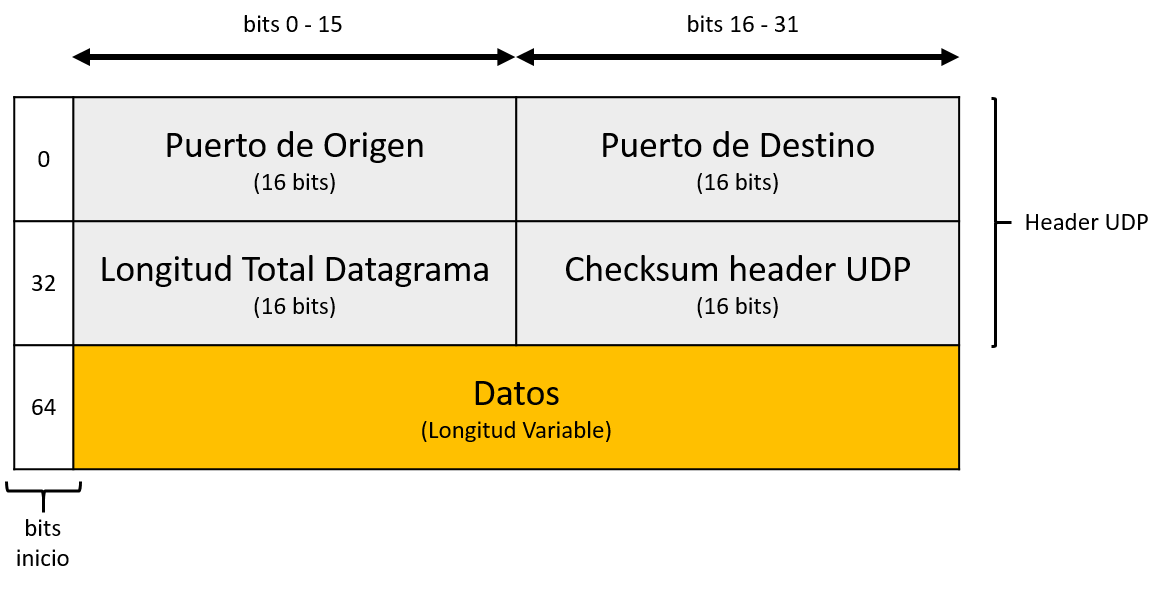
\includegraphics[scale=.55]{imagenes/estructuraUDP.png}
	\caption{Estructura de un paquete UDP con detalle del tamaño de sus encabezados de capa de transporte.}
	\label{fig:datagramaudp}
\end{figure}

El protocolo UDP se estandarizó el año 1980, sin embargo su aplicación ha sido muy variada en distintos sistemas modernos. Hoy por hoy UDP es uno de los componentes estructurales de la Internet estando presente en diversas aplicaciones que van desde transmisiones en uso intensivo de datos para redes de alta velocidad \cite{udp:highbandwidth}, hasta mecanismos de transmisión de video \cite{udp:video}, entre otros. Sin embargo, una de las aplicaciones más importantes (sino la más trascendental) de éste protocolo en la infraestructura de Internet, es su labor en el servicio DNS.

\subsection{DNS}
Todo dispositivo conectado a una red de computadoras se identifica a si mismo por la denominada \emph{dirección IP}, un identificador que permite referenciarlo y diferenciarlo de otros dispositivos conectados a la misma red, definido por el nivel 3 del modelo OSI. No obstante para poder conectarse con un recurso disponible en Internet, generalmente los dispositivos consultan por lo que llamamos \emph{nombres de dominio}, que son identificadores con carácter semántico para los usuarios que definen una red de identificación asociada a un grupo de dispositivos o equipos conectados a la red \cite{wiki:nombre_dominio}. Éste mecanismo de traducciones se conoce como \textbf{servicio DNS} y es vital para el funcionamiento de Internet como lo conocemos.

El servicio DNS \cite{rfc:1034, rfc:1035} opera como una base de datos distribuida que permite resolver consultas de manera jerarquizada basado en un principio de consultas recursivas. Frente a una consulta por un nombre de dominio, el primer paso es la resolución de la misma empleando datos de la caché local del servicio DNS del sistema (Esto es, emplear información previa en caso de que el nombre consultado ya hubiese sido preguntado anteriormente). En caso de encontrarse la respuesta en la caché local, se responde la consulta con ésta información y el proceso finaliza. En caso de que la consulta no coincida con algún registro local, se promueve el proceso de resolución de nombre al servidor DNS preferido (Configurado en el sistema).  

Frente a una consulta, un servidor DNS hace una verificación en su información local para determinar si tiene autoridad para responder al nombre solicitado en función de la zona que tenga configurada. En caso de que el nombre consultado coincida con algún registro de dicho servidor, el servidor usa ésta información para responder la consulta con autoridad y finaliza el proceso. En caso de que éste servidor no disponga de una entrada con el nombre pedido, se verifica en su caché local en caso de que previamente el servidor hubiese formado parte de una cadena de resolución para el nombre pedido, en cuyo caso puede responder con la resolución almacenada en caché y finalizar la consulta. Si tras todas las verificaciones anteriores (Sobre los registros de la zona DNS y de caché de resoluciones) el nombre de dominio consultado no registra apariciones en el servidor DNS preferido, la consulta se promueve recursivamente a otros servidores DNS con sugerencias de raíz para el nombre solicitado, de manera de poder conseguir una respuesta autoritativa en cada caso. Para esto la consulta se resuelve desde el dominio de nivel superior, resolviendo desde lo general a lo particular del nombre de dominio. Un ejemplo de resolución del dominio dcc.uchile.cl se ilustra en la imagen \ref{fig:dns}

\begin{figure}[!h]
	\centering
	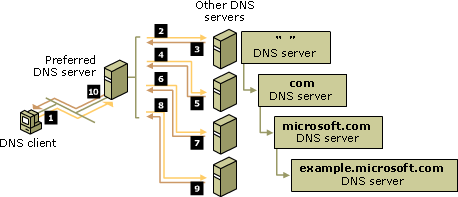
\includegraphics[scale=0.7]{imagenes/dns-system.png}
	\caption{Diagrama de operación del servicio DNS ilustrando comunicación entre servidores de dicho tipo.}
	\label{fig:dns}
\end{figure}

En la práctica, el servicio DNS emplea el protocolo UDP para la comunicación desde y hacia los servidores de dicho tipo, esto pues las características de una consulta DNS contemplan:

\begin{itemize}
\item \textbf{Consultas Auto-Contenidas} La información de una consulta DNS calza fácilmente en un paquete de UDP.
\item \textbf{Orden Irrelevante} Los requerimientos DNS no necesitan ser procesados en un orden establecido. Sin embargo, si requieren ser eventualmente procesados y ello en el menor tiempo posible. Un factor que justifica el uso de UDP al ser precisamente un protocolo orientado a mensajes.
\end{itemize}

De esta manera, las características anteriores justifican el uso de UDP como protocolo para la comunicación entre los servidores DNS.

El escenario antes descrito explica el por qué UDP tiene una participación de gran importancia en las redes actuales (en especial sobre Internet) y además, dado el sostenido aumento en el número de conexiones explicado en las secciones previas, da cuenta de cómo el tráfico de éste tipo de comunicación representa una porción muy significativa en la operación de las redes modernas. Una situación que con el paso de los años ha exigido cada vez mejores técnicas de procesamiento para dar mejores tiempos de respuesta.

\section{Sistemas Operativos Modernos}
El paso del tiempo ha permitido a los fabricantes de hardware desarrollar componentes cada vez de mayor capacidad. Procesadores, memorias, tarjetas de videos, sistemas de almacenamiento, y prácticamente todos los componentes de un computador han evolucionado en capacidad, un escenario que ha impulsado a los desarrolladores de sistemas operativos a generar plataformas más robustas y eficientes a la hora de aprovechar toda la nueva amalgama de recursos disponibles en cada nueva generación de componentes. Una de las características más notables para esta industria sin duda ha sido la \textbf{capacidad multiprocesador} o bien denominada \emph{SMP}\footnote{Por sus siglas en inglés: \textit{Symmetric Multi-Processor System}}.

A finales de la década de los 80, los fabricantes de microprocesadores hicieron uno de los saltos más significativos en la industria al promover una nueva arquitectura de hardware que postuló un nuevo enfoque de aprovechamiento del procesador, incorporando varios de los mismos en un esquema que planteaba como siguiente paso la idea de disponer múltiples procesadores en una máquina, de manera de delegar tareas para su ejecución simultánea. Éste enfoque permitió llevar a la práctica por primera vez la técnica del paralelismo en el software.

El primer enfoque arquitectural masivo para el paralelismo se denominó como la arquitectura \textbf{Front Side Bus} (FSB, ver figura \ref{fig:FSB}), muy popular entre procesadores de la línea Intel Core 2 Duo y Atom. Éste enfoque planteó la disposición de varios procesadores físicos, cada uno con recursos propios de memoria caché local los cuales se interconectaban por un canal de comunicación común, el cual daba acceso a la memoria completa del sistema y al resto de los recursos del mismo. El problema de ésta arquitectura era que para que un procesador pudiese emplear el bus de datos, necesariamente el mismo debía estar libre de comunicaciones de cualquier otro procesador, problema que al poco tiempo que las memorias aumentaron su capacidad evidenció un efecto de cuello de botella inherente a éste diseño.

\begin{figure}[th!]
\centering
\subfigure[Arquitectura \emph{FSB}]{
	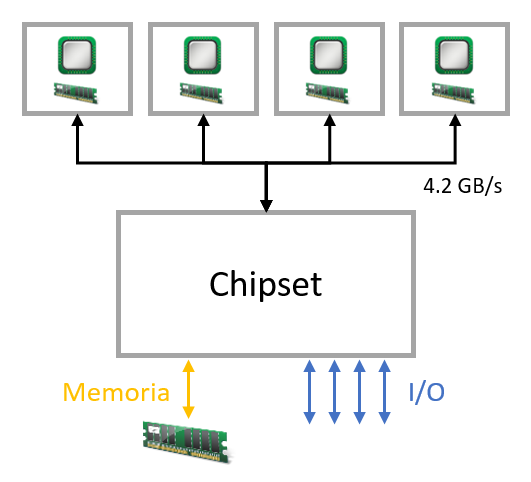
\includegraphics[width=.3\textwidth]{imagenes/FSB.png}
	\label{fig:FSB}
}
\subfigure[Arquitectura \emph{DIB}]{
	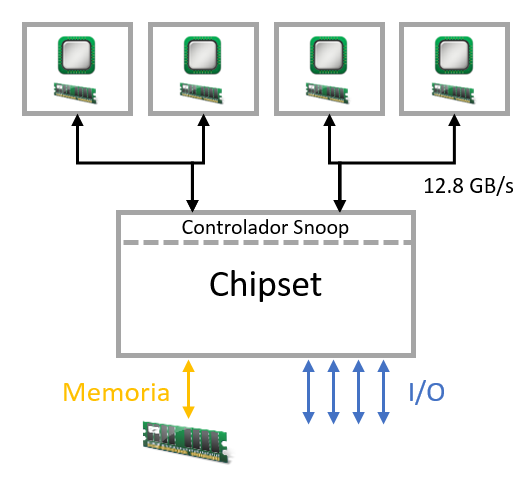
\includegraphics[width=.3\textwidth]{imagenes/DIB.png}
	\label{fig:DIB}
}
\subfigure[Arquitectura \emph{DHSI}]{
	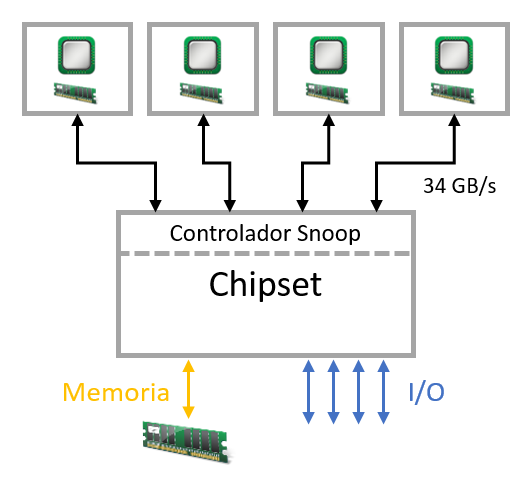
\includegraphics[width=.3\textwidth]{imagenes/DHSI.png}
	\label{fig:DHSI}
}
\caption{Diagrama de las distintas arquitecturas de hardware para la comunicación de múltiples procesadores.}
\label{fig:arquitecturas}
\end{figure}

Con objeto de explotar mejor el potencial de un esquema multiprocesador se desarrollaron varios rediseños del esquema FSB con el fin de eliminar el punto de contención en el bus compartido. Así es como surgieron las arquitecturas \textbf{Dual Independent Bus} y \textbf{Dedicated High-Speed Interconnects} (imagen \ref{fig:DIB} y \ref{fig:DHSI} respectivamente) que postulan un enfoque similar a FSB pero garantizando un canal exclusivo para cada procesador o grupo de procesadores del sistema. Una mejora inmediata de estos enfoques con respecto a FSB corresponde a un significativo aumento de las velocidades de transferencia, esto de la mano de que con canales cada vez más exclusivos por CPU se consiguen mejores velocidades en la comunicación general. Sin embargo, estas modificaciones revelaron otro aspecto a considerar: En sistemas SMP, y básicamente en cualquier sistema que teóricamente plantee la capacidad de procesamiento paralelo, deben haber mecanismos de control de consistencia de los datos que permitan mantener un registro coherente de los valores almacenados en distintas porciones del sistema. Vale decir, como los esquemas de procesamiento múltiple emplean procesadores provistos tanto de memoria local como de memoria compartida, se deben emplear mecanismos que garanticen la consistencia y coherencia de los valores que tengan presencia en diferentes locaciones del sistema. A dicho conjunto de esquemas de control de valores se les denomina \emph{protocolos de coherencia de cache} y son los que dan flexibilidad en un sistema para que la memoria local de un procesador disponga de valores coherentes con la más reciente modificación de dicho valor, aun habiendo ocurrido ésta modificación en otro núcleo de procesamiento.

\begin{figure}[!h]
	\centering
	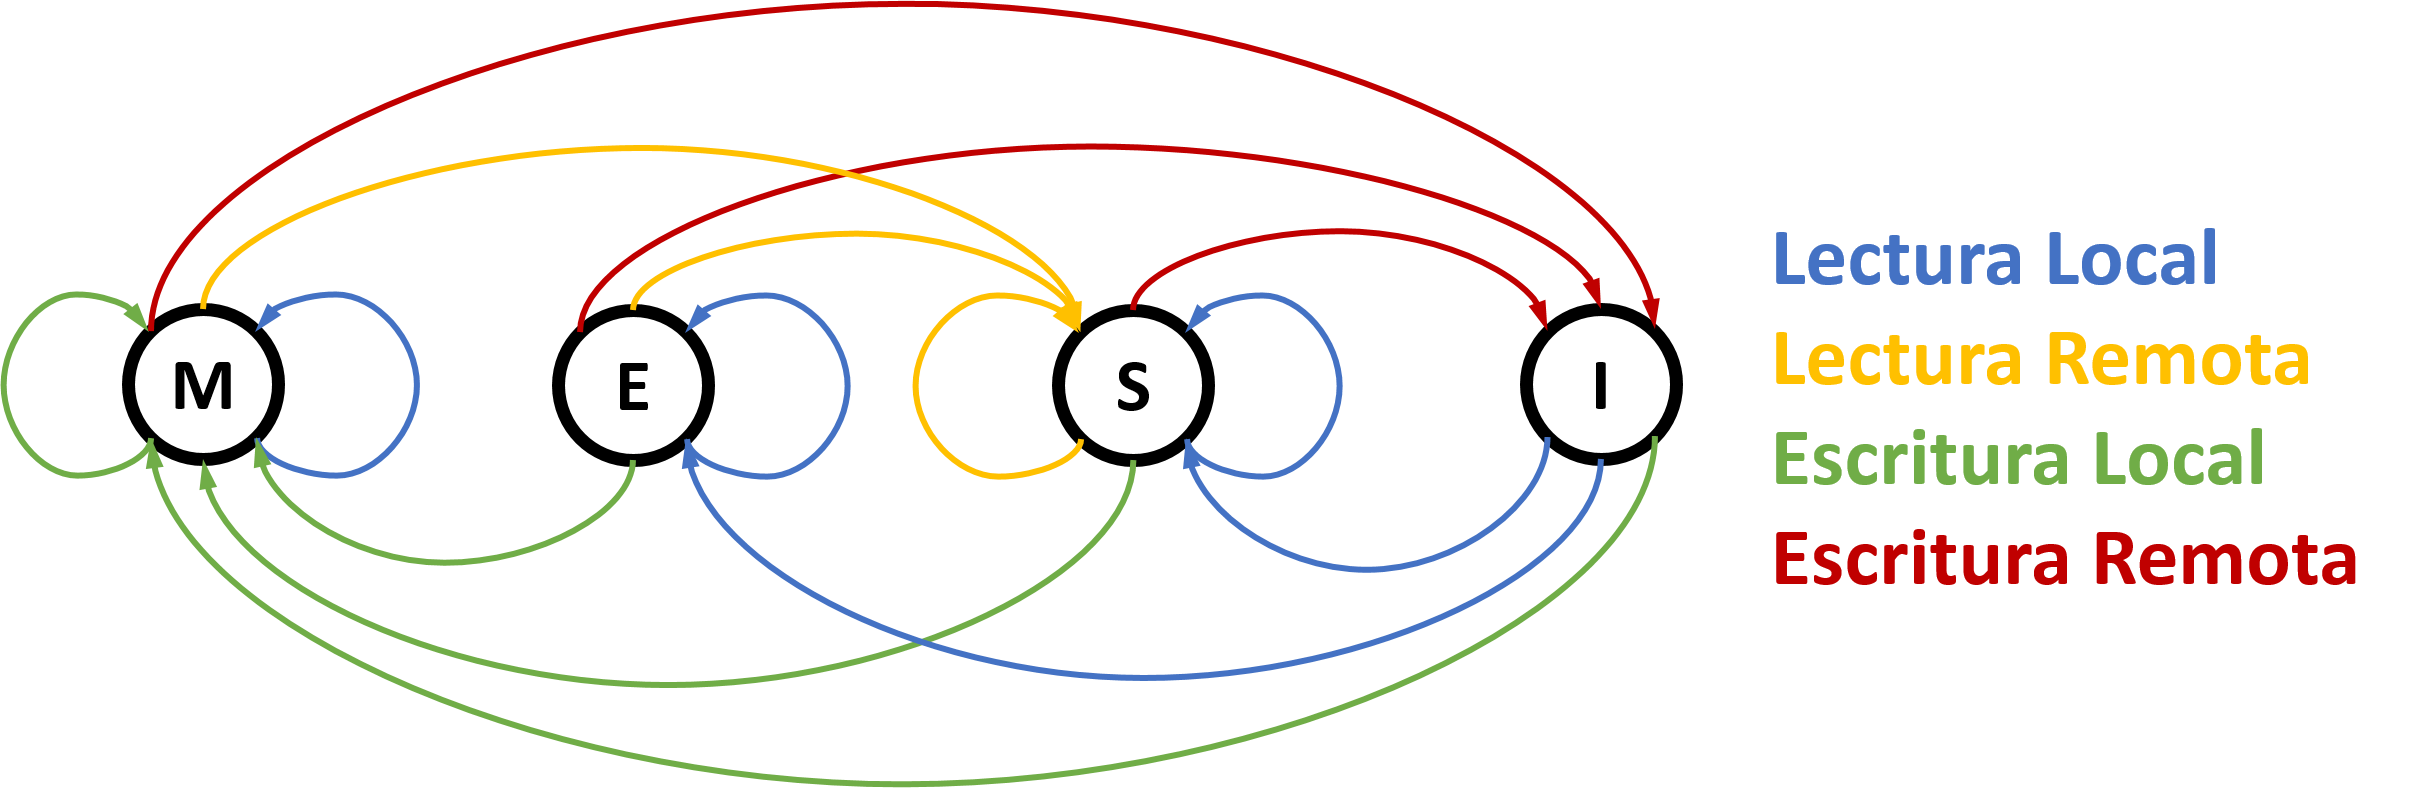
\includegraphics[scale=0.3]{imagenes/MESI.png}
	\caption{Diagrama de transiciones del protocolo MESI.}
	\label{fig:MESI}
\end{figure}

%\begin{center}
%\begin{tikzpicture}[scale=0.13]
%\tikzstyle{every node}+=[inner sep=0pt]
%\draw [black] (10.3,-21.8) circle (3);
%\draw (10.3,-21.8) node {$M$};
%\draw [black] (29.9,-21.8) circle (3);
%\draw (29.9,-21.8) node {$E$};
%\draw [black] (50.5,-21.8) circle (3);
%\draw (50.5,-21.8) node {$S$};
%\draw [black] (70.6,-21.8) circle (3);
%\draw (70.6,-21.8) node {$I$};
%\draw [black] (11.517,-19.059) arc (153.39789:26.60211:32.358);
%\fill [black] (69.38,-19.06) -- (69.47,-18.12) -- (68.58,-18.57);
%\draw [black] (9.739,-24.735) arc (16.90501:-271.09499:2.25);
%\fill [black] (7.63,-23.14) -- (6.72,-22.89) -- (7.01,-23.85);
%\draw [black] (52.948,-20.074) arc (119.61129:60.38871:15.386);
%\fill [black] (68.15,-20.07) -- (67.7,-19.24) -- (67.21,-20.11);
%\draw [black] (31.697,-19.4) arc (139.64058:40.35942:24.348);
%\fill [black] (68.8,-19.4) -- (68.67,-18.47) -- (67.9,-19.11);
%\draw [black] (68.363,-23.79) arc (-54.70403:-125.29597:13.522);
%\fill [black] (52.74,-23.79) -- (53.1,-24.66) -- (53.68,-23.84);
%\draw [black] (68.442,-23.882) arc (-49.11238:-130.88762:27.792);
%\fill [black] (32.06,-23.88) -- (32.34,-24.78) -- (32.99,-24.03);
%\draw [black] (51.823,-24.48) arc (54:-234:2.25);
%\fill [black] (49.18,-24.48) -- (48.3,-24.83) -- (49.11,-25.42);
%\draw [black] (49.177,-19.12) arc (234:-54:2.25);
%\fill [black] (51.82,-19.12) -- (52.7,-18.77) -- (51.89,-18.18);
%\draw [black] (32.324,-20.04) arc (120.44489:59.55511:15.543);
%\fill [black] (48.08,-20.04) -- (47.64,-19.2) -- (47.13,-20.07);
%\draw [black] (12.237,-19.511) arc (136.33228:43.66772:25.109);
%\fill [black] (48.56,-19.51) -- (48.37,-18.59) -- (47.65,-19.28);
%\draw [black] (28.577,-19.12) arc (234:-54:2.25);
%\fill [black] (31.22,-19.12) -- (32.1,-18.77) -- (31.29,-18.18);
%\draw [black] (7.601,-20.517) arc (272.30317:-15.69683:2.25);
%\fill [black] (9.68,-18.88) -- (10.14,-18.06) -- (9.15,-18.1);
%\draw [black] (12.857,-20.239) arc (116.16519:63.83481:16.425);
%\fill [black] (12.86,-20.24) -- (13.8,-20.34) -- (13.35,-19.44);
%\draw [black] (48.372,-23.913) arc (-48.37501:-131.62499:27.057);
%\fill [black] (12.43,-23.91) -- (12.69,-24.82) -- (13.36,-24.07);
%\draw [black] (69.21,-24.458) arc (-30.18959:-149.81041:33.273);
%\fill [black] (11.69,-24.46) -- (11.66,-25.4) -- (12.52,-24.9);
%\end{tikzpicture}
%\end{center}


En lo que a estos protocolos respecta, el más popular en los sistemas modernos es el denominado protocolo \textbf{MESI}\footnote{También se le denomina protocolo Illinois, en sentido de la universidad del mismo nombre.} \cite{paper:MESI}, denominado así por las iniciales de las palabras en inglés: \textbf{M}odified (Modificado), \textbf{E}xclusive (Exclusivo), \textbf{S}hared (Compartido) e \textbf{I}nvalid (Inválido). Es un protocolo que plantea un diagrama de estado (basado en los 4 estados que componen su nombre) para cada linea de memoria caché con información almacenada, a modo de mantener su integridad en el sistema frente a modificaciones que realice algún procesador (ya sea dueño de dicho banco de memoria o no). En conjunto con el protocolo \emph{MESI} existe la técnica \textbf{Buss Snooping} \cite{paper:snoop} que consiste en un esquema de coordinación para interceptar, notificar, modificar y coordinar los valores de memoria a medida que se van realizando cambios de los mismos por una determinada tarea. En conjunto, el protocolo \emph{MESI} y la operación del \emph{Bus Snooping} hacen posible las operaciones paralelas en entornos multiprocesador, proveyendo un ambiente adecuado para programar aplicaciones con ejecución verdaderamente paralela al brindar una capa de abstracción suficientemente flexible para aprovechar ésta técnica.

\subsection{Programación Multi-Hilo}
En la práctica, existen distintas maneras de conseguir paralelismo a la hora de programar un sistema. Los dos enfoques tradicionales es pensar en esquemas \textbf{multiproceso} (denominados procesos pesados) y \textbf{multihilo} (denominados procesos ligeros), diferenciados principalmente porque los primeros disponen de espacios de memoria disjunto entre ellos, no así los segundos. La programación multi-hilo es muy usada en aplicaciones por ser un enfoque probado y de fácil adopción por el soporte que brindan los sistemas operativos modernos a través de librerías que incorporan llamadas a sistema para tales fines, una la más populares en entornos UNIX es \textbf{PThreads}.

PThreads\footnote{Especificación base de la IEEE \url{http://pubs.opengroup.org/onlinepubs/9699919799/basedefs/pthread.h.html}} (o \emph{POSIX Threads} de su nombre completo) es una interfaz prácticamente estándar de programación hoy entre sistemas UNIX, resultado del trabajo de diseñadores de sistemas operativos que a finales de los 80 se abocaron al desarrollo de sistemas escalables para las nuevas arquitecturas de multiprocesadores. Ésta interfaz provee funciones para gatillar y controlar hilos de ejecución creados a partir de un proceso padre. Los hilos se caracterizan por disponer de un espacio de memoria propio cada uno con información privada (Con valores como el puntero de instrucciones, el \emph{Stack} de memoria, etc.) además de compartir entre ellos otros elementos como  por ejemplo el espacio de direccionamiento, señales del sistema o descriptores de archivos, característica que permite cierta comunicación entre ellos. Son una forma liviana de proveer paralelismo con respecto a su símil multiproceso provista por las llamadas a sistema \verb=fork()= y \verb=exec()= que generan tareas con espacios de memoria disjuntos entre ellas. Aún siendo procesos denominados ``ligeros'' y de incorporar ciertas dificultades a la hora de concebir el diseño de una aplicación, el uso de hilos a la hora de programar permite postular a un importante beneficio como lo es la escalabilidad en sistemas multiprocesador, ello al permitir que los distintos hilos se ejecuten en distintos procesadores físicos logrando ganancias efectivas en los tiempos netos de ejecución al distribuir la carga en distintos núcleos de procesamiento.

En contraparte con lo anterior, la programación concurrente conlleva ciertas dificultades inherentes a su capacidad de ejecución simultánea. Quizá el desafío más importante sea que obliga a cambiar el diseño de las aplicaciones, haciendo necesario la aplicación de criterios sofisticados para resolver problemas de sincronización y de acceso a secciones críticas que son inherentes a éste modelo de programación.


\subsection{Mecanismos de Sincronización del Sistema}
Una responsabilidad fundamental de los sistemas operativos modernos es asignar el uso de recursos a las aplicaciones y garantizar un entorno seguro para la ejecución de dichas aplicaciones en el sentido del acceso a datos o recursos del sistema. En ésta línea, garantizar \textbf{consistencia en los datos} es una labor crucial en esquemas modernos, capaces de generar escenarios de múltiples aplicaciones con acceso simultáneo a datos compartidos entre ellas. La característica de operaciones paralelas es una introducción al kernel de Linux desde su versión 2.6\footnote{En versiones previas del kernel, la operación por defecto del \emph{scheduler} del kernel era serializar las tareas con accesos simultáneos al sistema.} que apareció a la vez que se popularizaron los equipos con capacidad multi-procesador, lo cual introdujo un nuevo nivel de complejidad en la labor de los sistemas operativos, haciéndolos responsables de mantener la correcta consistencia de la información en los distintos niveles de memoria en un escenario de ejecuciones paralelas, problema conocido típicamente como de \emph{Secciones Críticas} \colorbox{yellow}{[AKA una referencia a algo que estudie solo el tema de secciones criticas]}.

Para proveer operaciones sobre los datos en escenarios concurrentes, los sistemas operativos modernos implementan mecanismos de sincronización que permiten garantizar consistencia en sus estructuras de datos, permitiendo así operaciones simultáneas sobre una determinada estructura, y brindando así el efecto de compartir una estructura entre distintos procesos para que la modifiquen coincidentemente. Procesos que en la práctica pueden estar ejecutándose en núcleos de procesamiento distintos.

Para ello, el hardware de las computadoras provee las denominadas \emph{Operaciones Atómicas de Bajo nivel}, que son un conjunto de herramientas básicas que permiten manejar escenarios de concurrencia. Éstas mismas operaciones ya provistas son la base para las denominadas \emph{Primitivas de Sincronización de Alto Nivel}, las cuales son cruciales para la correcta implementación de programas multi-hilo o multi-proceso. A continuación se repasan las diferencias conceptuales entre cada tipo de primitiva de sincronización y se mencionan las implementaciones más importantes de cada una que atañen a la presente investigación \cite{book:SOConcepts}.

\begin{table}[]
\centering
\begin{tabular}{|c|c|}
\hline
\textbf{\begin{tabular}[c]{@{}c@{}}Primitivas de sincronización\\ de Bajo Nivel\end{tabular}} & \textbf{\begin{tabular}[c]{@{}c@{}}Primitivas de sincronización\\ de Alto Nivel\end{tabular}} \\ \hline
Memory barrier & Completion                                                                                    \\ \hline
Atomic operations & Semaphore                                                                                     \\ \hline
Synchronize with interrupts & Futex                                                                                         \\ \hline
Spin locks & Mutex                                                                                         \\ \hline
\end{tabular}
\caption{Algunos ejemplos de herramientas de sincronización de distinto nivel disponibles en sistemas Linux.}
\label{tab:syncTools}
\end{table}

\subsubsection{Operaciones Atómicas}
Corresponden a un conjunto de instrucciones provistas por hardware disponibles en ambientes multi-procesador las que, aun siendo ejecutadas simultáneamente en distintas CPU's, en la práctica son ejecutadas secuencialmente en un orden arbitrario. En éste caso la exclusión mutua es provista usando variables de naturaleza \verb=boleanas= que se denominan \emph{lock}. Existen diversas implementaciones de operaciones de éste tipo siendo las más conocidas: \emph{Test-and-Set}, que valida una condición y si se cumple realiza una asignación, \emph{Swap}, que intercambia el valor contenido entre dos variables, etc.

\subsubsection{Semáforo}
La solución a la protección de secciones críticas provista por mecanismos de operaciones atómicas es difícil de generalizar para aplicaciones más complejas, como en el caso en que se tienen múltiples hilos de ejecución. En este punto, se emplea una nueva herramienta de sincronización: Los \emph{Semáforos}. Un semáforo es una estructura de sistema que lleva una cuenta de un entero que puede ser modificado por medio de las operaciones atómicas \emph{Wait} y \emph{Signal}, que permiten verificar una condición para luego hacer un decremento del contador interno del semáforo, y gatillar un incremento de dicho contador, respectivamente.

Para su uso, la idea es que los diferentes hilos o procesos paralelos que soliciten acceso a un recurso compartan una estructura semáforo que sirva como barrera de acceso al recurso mismo. El semáforo admite la entrada de nuevos hilos de ejecución a la sección crítica protegida mientras su contador sea mayor que cero. De ésta manera un proceso que no consigue acceso al recurso protegido por un semáforo cae en un estado de espera (o a modo dormido) donde no gasta recursos del sistema.

\subsubsection{Mutex}
Los \textbf{Mutex} -o Monitores en español- Son otra estructura de sincronización de alto nivel provista por el propio kernel (disponible en \verb=kernel/locking/mutex.c=). Su nombre es precisamente la sigla en inglés de \emph{\textbf{Mut}ual \textbf{Ex}clusion Object}, que provee una herramienta para dar exclusión mutua en acceso a un recurso. En la práctica, corresponde a un semáforo binario, permitiendo el acceso exclusivo de un hilo de ejecución a un recurso protegido.

\subsubsection{SpinLock}
Son las primitivas de sincronización de más bajo nivel disponible en los sistemas Linux para garantizar exclusión mutua. Su operación se basa en ciclos de espera denominados \emph{busy-waiting} que son ciclos de procesador muertos, donde no se hace más que verificar el cambio de una condición que en la práctica consiste en ``obtener'' el \emph{lock}. Esta lógica de operación hace de los spinlocks una herramienta de sincronización de cuidado pues su operación está pensada solo para secciones críticas ligeras (de pocas instrucciones). Se diferencia de las otras herramientas de sincronización pues es usada en entornos de código que no puede dormir y debe estar preparado para retomar su operación\footnote{Un ejemplo de éste tipo de códigos son los \textit{Handlers} de interrupciones, que deben estar siempre listos para manejar un evento.}. Los sistemas operativos modernos proveen ésta estructura de sincronización y una completa interfaz de uso, disponible desde sus encabezados en \verb=include/linux/spinlock.h=.

Bien utilizados, los spinlocks son capaces de proveer un mejor desempeño que las otras estructuras revisadas. Por el contrario, es sabido que el mal uso de éste tipo de herramientas de sincronización produce degradaciones importantes en los tiempos de operación generales de todo el sistema, pues significa el consumo de recursos en ciclos de procesamiento desperdiciados sin trabajo real, lo que en la práctica se traduce en un bloqueo de un hilo de ejecución \cite{paper:nonscalablelocks, paper:cachebouncing}. Aun cuando las implementaciones modernas de sistemas operativos incluyen optimizaciones en el rendimiento de éstas estructuras (ya sea con optimizaciones energéticas o mejoras de scheduling \cite{paper:cacheaffinity}) lo cierto es que la naturaleza inherente para brindar sincronización de los spinlocks es por medio del mecanismo de \emph{busy-waiting}, que significa desperdiciar ciclos de reloj sólo esperando.

Los spinlocks son una de las estructuras de sincronización preferidas a la hora de solucionar escenarios de concurrencia en otras estructuras desplegadas en el kernel\footnote{Empleadas en módulos del kernel, colas de datos y}, siempre tratando de mantener el cuidado de resguardar sólo regiones de código acotadas que no arriesguen el desempeño general del sistema en contextos de concurrencia.


\subsection{Sockets en Linux}
El modelo OSI ha estipulado a la familia de los protocolos TCP/IP como un estándar a la hora de establecer mecanismos de conexión entre computadoras. Sin embargo, las interfaces de programación no siguen la misma naturaleza estándar. Los distintos sistemas operativos implementan distintas interfaces públicas de aplicación (APIs) para el uso práctico de TCP/IP. \textbf{Socket} es la denominación tradicional para las interfaces de programación que proveen los mecanismos para realizar tales conexiones. En otras palabras, es la interfaz que provee el sistema operativo para enviar mensajes a través de la red. En la práctica un socket representa una interfaz o punto de comunicación que maneja un protocolo de comunicación especifico. Los sockets operan bajo una dinámica denominada \emph{Cliente/Servidor} que especifica que la comunicación debe ser originada por un cliente y atendida posteriormente por un servidor, en ese orden.

Los sockets en Linux \cite{rfc:147, book:sockets} son estructuras que se construyen por medio de la llamada de sistema \verb=socket()=. Son estructuras provistas por el kernel del sistema\footnote{Típicamente implementada e importada desde el prototipo \verb=<sys/socket.h>=, disponible en los encabezados del kernel.} que al utilizarlos se manejan simplemente como descriptores de archivo, a pesar de que en su implementación a bajo nivel son bastante más complejos que una interfaz de sólo entrada y salida de datos. La gran diferencia de los sockets de Linux con respecto al común de mecanismos de entrada/salida por archivos es que los sockets están concebidos para una operación basada en un principio \emph{Cliente-Servidor}, lo que impacta finalmente en que su descriptor no apunta directamente a un archivo y su utilidad queda determinada sólo desde el momento en que se complete la dinámica de llamadas a sistema que hagan se establezca una conexión efectiva, ello dependiendo del protocolo a usar (Ver imagen \ref{fig:socketHandshake}). Linux cuenta con una API que provee métodos de comunicación sencillos para la manipulación de los sockets de acuerdo al protocolo para el que se configure el mismo.

\begin{figure}[h!]
	\centering
	\hspace*{\fill}
	\subfigure[Llamadas de sistema en esquemas de comunicación orientados a la conexión, como el caso de TCP.]{
		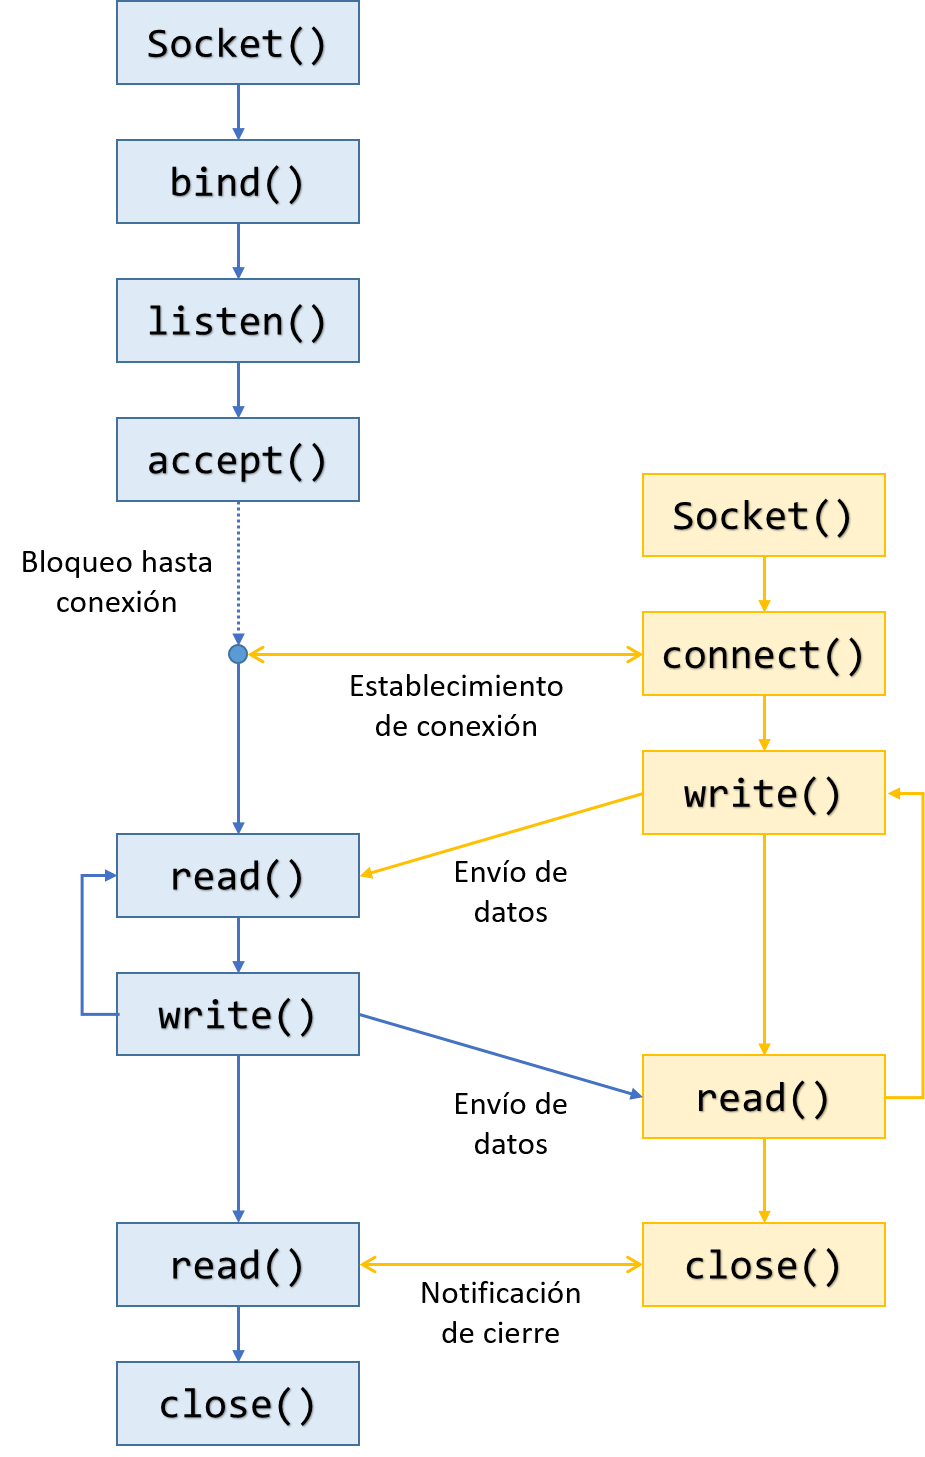
\includegraphics[width=.4\textwidth]{imagenes/llamadasTCP.png}
	}\hfill
	\subfigure[Llamadas de sistema en esquemas de comunicación orientados a la mensajería, como el caso de UDP.]{
		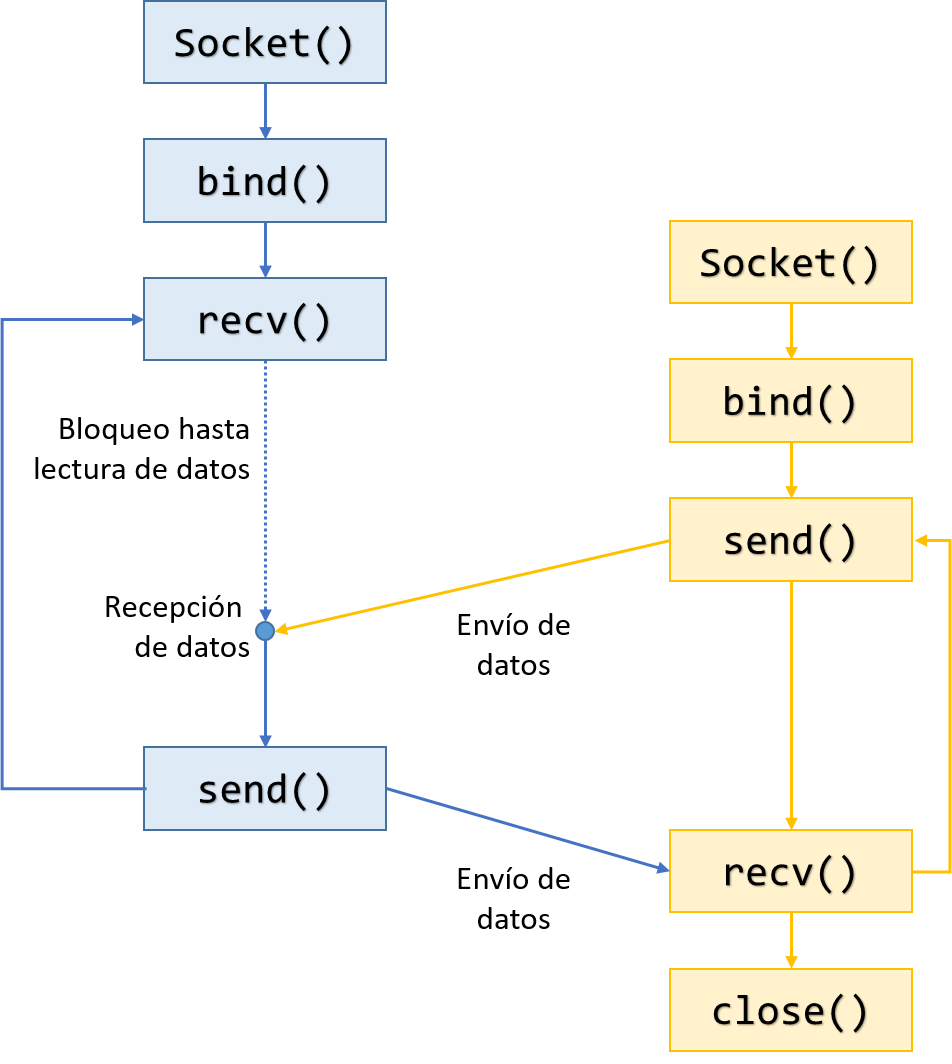
\includegraphics[width=.4\textwidth]{imagenes/llamadasUDP.png}
	}
	\caption{Un esquemático de las llamadas a sistema que se deben suceder para establecer una conexión \cite{book:sockets}. En éste caso, los componentes amarillos representan el lado cliente y aquellos azules representan el lado servidor en la dinámica de conexión.}
	\label{fig:socketHandshake}
	\hspace*{\fill}
\end{figure}


El sistema operativo reconoce a los diferentes sockets en operación a través de sus detalles de conexión de red, ello por medio de tuplas que contienen información de la conexión que provee el mismo. Una tupla congrega datos como: El protocolo de comunicación, las direcciones local y remota (con información de las capas de red y de transporte para la identificación del punto de acceso) y los identificadores de procesos local y remoto propietarios del punto de comunicación.

Los sockets son elementos muy versátiles en cuanto a su manipulación y uso. Se pueden usar en dos variantes principales que determinan el \emph{dominio del socket}:
\begin{description}
\item[Unix Sockets] Corresponden a un tipo de punto de comunicación que proveen los sistemas UNIX para realizar comunicación entre procesos de un mismo host.
\item[Internet Sockets] Son otro tipo de sistema de puntos de comunicación provistos en sistemas UNIX, basados en proveer una interfaz simple para implementar mecanismos de comunicación sobre una red.
\end{description}

Para las variedades recién mencionadas hay que sumar la capacidad de configuración de un socket. La primera y más importante es la configuración del modo de conexión que rige la dinámica de comunicación del socket: El \emph{protocolo de comunicación}. En éste apartado existen dos variantes comúnmente usadas: \verb=SOCK_STREAM= y \verb=SOCK_DGRAM= para usar TCP o UDP respectivamente. Sumado a lo anterior, los sistemas Linux proveen de la llamada de sistema \verb=setsockopt= que permite modificar características de una instancia socket, activando ciertas funcionalidades específicas o habilitando implementaciones con modificaciones especiales con respecto al funcionamiento estándar.

Más allá de la configuración puntual de la que se dote a un socket, la estructura interna de éste elemento es estándar y tiene especificaciones importantes de comentar para comprender su funcionamiento y posibles limitaciones.


\subsubsection{Estructura Interna}
Los socket de Linux están definidos como una estructura en el núcleo del sistema en \verb=include/linux/net.h= (ver figura \ref{fig:socketAnathomy}). En primera instancia, esta estructura incluye datos de su estado, información de su funcionamiento activo, etc. E incorpora dos sub estructuras fundamentales: \verb=proto_ops= que hace un nexo de punteros para con todas a aquellas funciones relacionadas a la manipulación del socket en su interacción de funcionamiento, implementando las funcionalidades mismas del socket. Y \verb=sock=, que contiene otras estructuras importantes en el funcionamiento correcto del socket, por ejemplo, estructuras usadas para el tránsito de los paquetes que por ellos circulan. Definida en ésta última estructura, cada socket posee 3 colas de tránsito que se usan para los procesos de encolamiento y desencolamiento de paquetes al socket mismo:
\begin{description}
\item[Receive\_queue] Cola de almacenamiento para los paquetes recién arribados al socket.
\item[Write\_queue] Cola de almacenamiento de los paquetes previo al envío de los mismos por la conexión definida por el socket.
\item[Backlog\_queue] Cola de almacenamiento de paquetes usada para colectar paquetes recibidos cuando la \textbf{Receive\_queue} está bloqueada (ocupada).
\end{description}

\begin{figure}[!h]
	\centering
	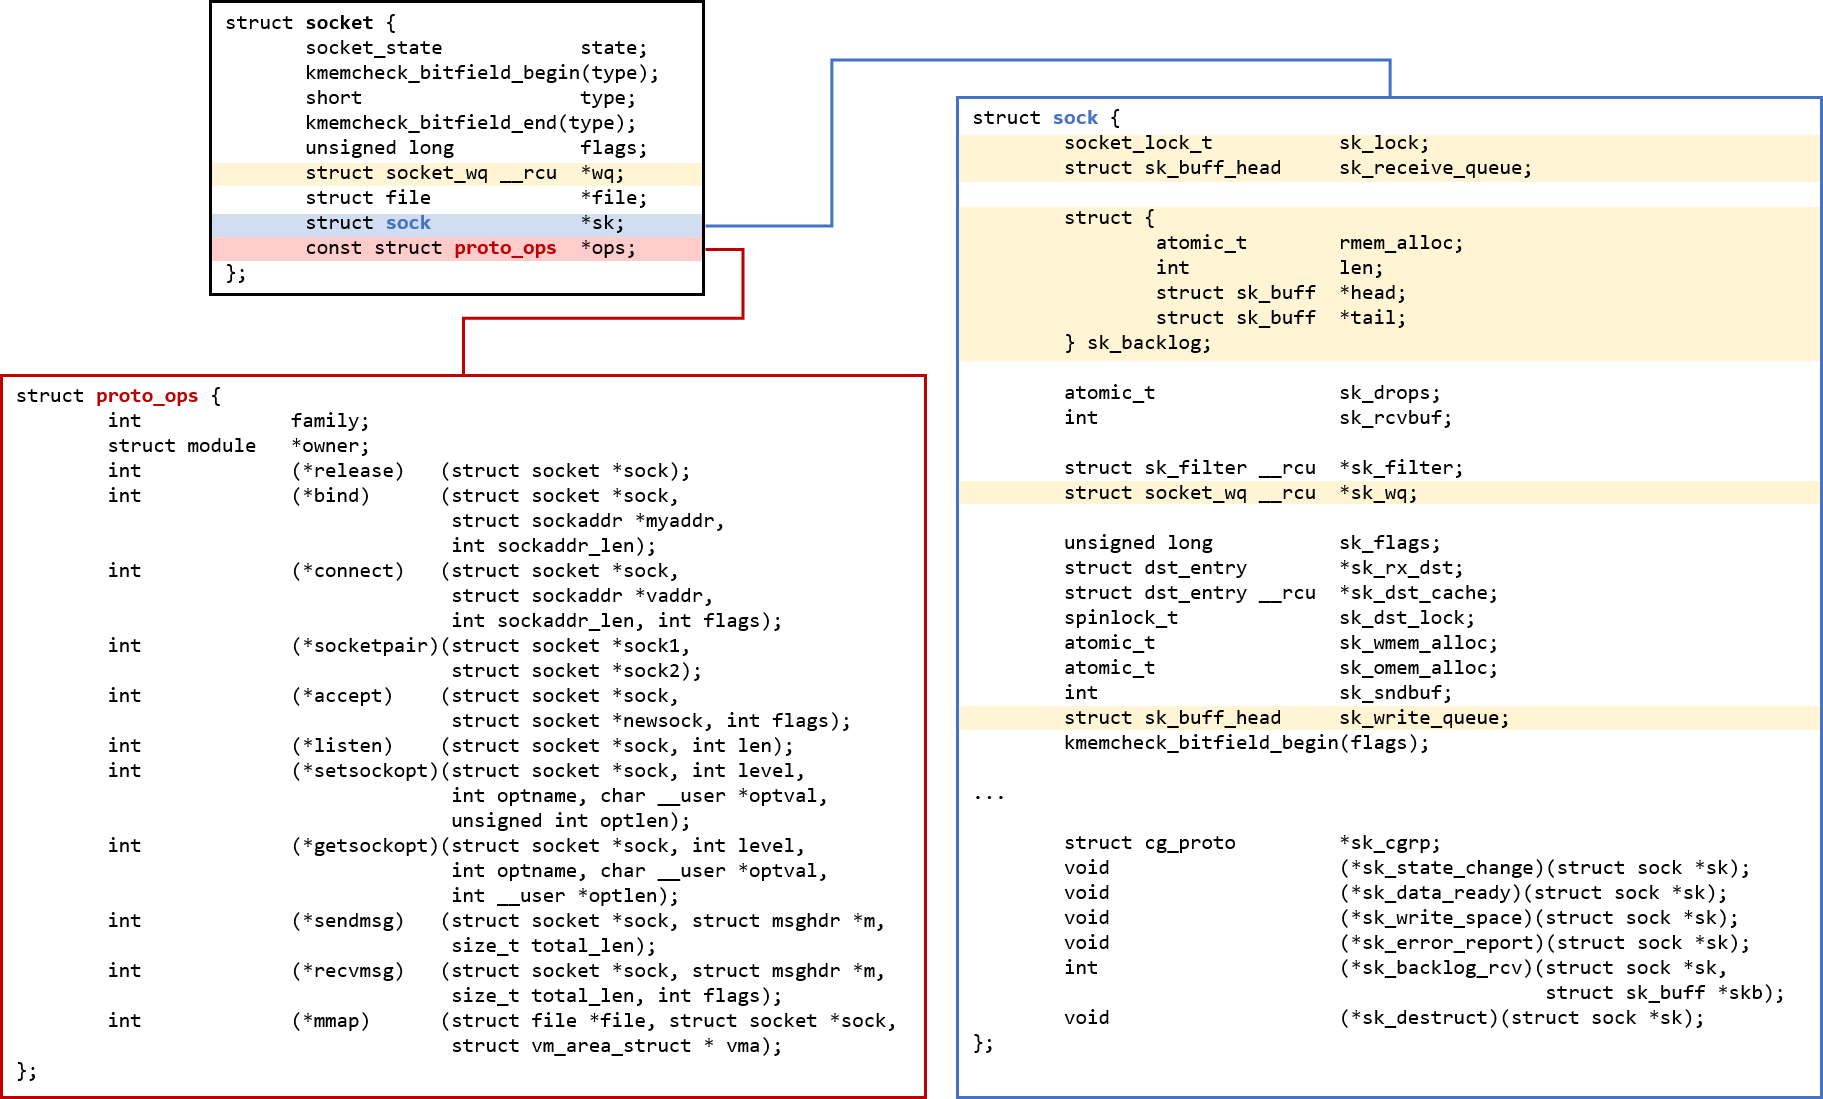
\includegraphics[scale=0.53]{imagenes/socketStructsDependecy.png}
	\caption{Diagrama de dependencias de la estructura interna de un Internet socket de Linux.}
	\label{fig:socketAnathomy}
\end{figure}

En términos de sus protecciones, los Internet sockets emplean spinlocks como herramientas de sincronización en el acceso a las estructuras internas que participan en los procesos de encolamiento y desencolamiento de paquetes (Ver figura \ref{fig:socketAnathomy2}). Específicamente, se reconocen dos capas de protección: Una primera capa, dada por un spinlock general en el acceso al socket, y una segunda protección dada por limitaciones en el acceso a las colas de tránsito los paquetes. Cada una de las 3 colas antes mencionadas posee su propio spinlock de protección frente a modificaciones concurrentes en pos de garantizar la integridad y coherencia de las operaciones sobre la misma.

\begin{figure}[!h]
	\centering
	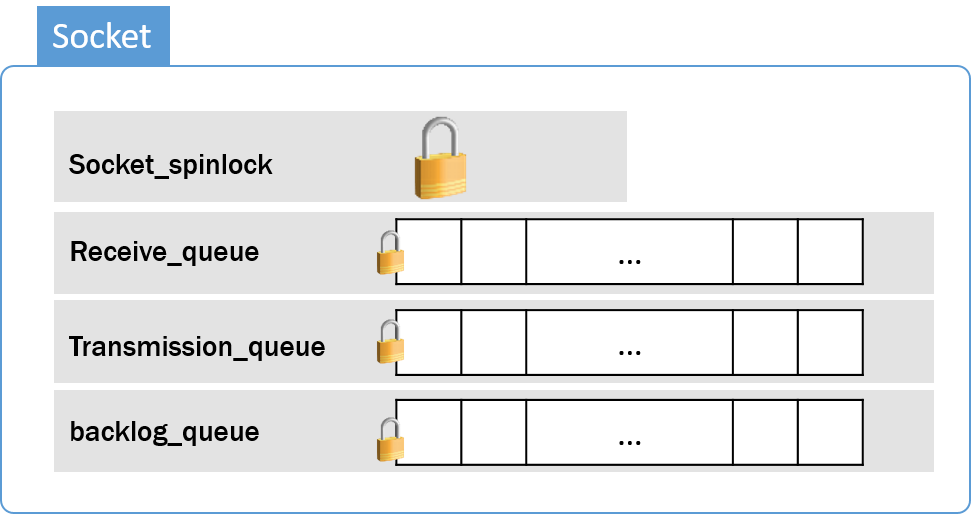
\includegraphics[scale=0.6]{imagenes/spinlocksSocket.png}
	\caption{Diagrama de niveles de protección presentes en un Internet socket de Linux.}
	\label{fig:socketAnathomy2}
\end{figure}

Por otro lado, el tránsito de un paquete que circula camino a un host puede ser descrito en una secuencia de pasos lógicos en que se interviene el mismo desde su arribo por una interfaz de red al llegar al socket:
\begin{enumerate}
\item Bloquear el socket usando el spinlock general de la estructura. De ésta manera se limitan las interrupciones para evitar concurrentemente encolamiento de otros paquetes.
\item Verificar si el lock está siendo usado por alguna aplicación de nivel usuario, en cuyo caso, se realiza el encolamiento del paquete directamente en la \textbf{Backlog\_queue}. Luego, para cada paquete:
	\begin{enumerate}
	\item Es procesado de acuerdo a las reglas de \emph{Netfilters}
	\item Son actualizadas las estadísticas del sistema, como \emph{Memory Accounting}.
	\item Se realiza el ingreso a la \textbf{Receive\_queue} (Esperando hasta la disponibilidad de su spinlock).
	\item Se hace una llamada al \emph{Scheduller} del sistema, para retomar procesos dormidos que hayan solicitado paquetes a éste socket.
	\end{enumerate}
\item Finalmente, se libera el spinlock general, continuando el proceso de recepción de los paquetes siguientes.
\end{enumerate}

\section{Presentación del Problema}
Como ya se mencionó, el escenario advertido para los próximos años prevé un inmenso tráfico a Internet que podría llevar la cantidad de procesamiento del servicio DNS a varios órdenes de magnitud por encima de la carga actual. Es más, el panorama futuro postula que los dispositivos más avanzados serían muchísimo más versátiles en su operación pudiendo hacer un uso más agresivo y demandante de la red, realidad que se traduciría en más conexiones.

En este contexto, el servicio DNS --como pieza estructural de Internet-- debe estar preparado para enfrentar de la mejor manera posible la gran carga de procesamiento antes señalada, sobre todo dado que --por su naturaleza jerárquica-- éste servicio escala rápidamente el tráfico entre servidores. En estricto rigor, el sistema de DNS debe garantizarse eficiente en cualquier escenario.

A modo de preparativo para el escenario anterior, distintas instituciones han trabajado en alternativas para mejorar el procesamiento de las peticiones DNS a fin de optimizar su operación y tiempos de respuesta. Una apuesta para otorgar dicha mejora en performance y en línea con la tendencia actual de multiplicar el poder de procesamiento añadiendo más núcleos, consiste en incorporar paralelismo en el procesamiento de las consultas. Para ello se propone un esquema como el detallado en el diagrama de la ilustración \ref{fig:multi_thread} donde la idea consiste en que una misma maquina DNS pueda atender múltiples solicitudes de manera simultánea a través de una misma interfaz de red (en nuestro caso, un socket UDP). Este enfoque supone como principal mejora el escalamiento del procesamiento de peticiones DNS en un factor proporcional a la cantidad de hilos de ejecución atendiendo la interfaz compartida, ello siempre y cuando existan núcleos reales de procesamiento disponibles para los distintos hilos. 

\begin{figure}[!h]
	\centering
	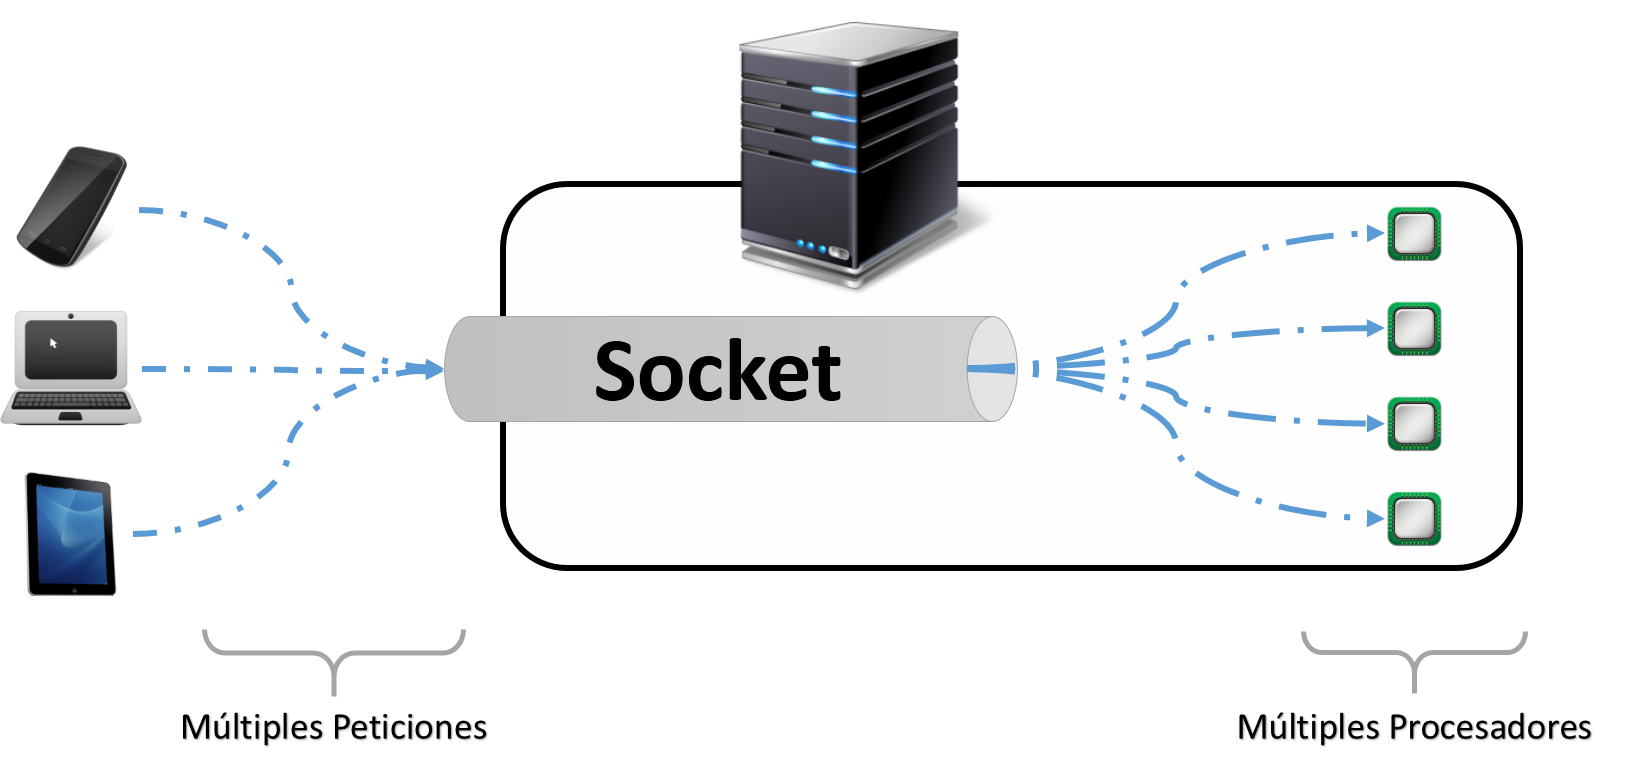
\includegraphics[scale=0.45]{imagenes/conf_multi_thread}
	\caption{Esquema de procesamiento multi-thread en un servidor con 4 procesadores reales, empleando un hilo por procesador. Escenario que en teoría, supone un mejor desempeño general, más no lo consigue en la práctica.}
	\label{fig:multi_thread}
\end{figure}

Inspirados en la consistencia del argumento teórico detrás de la propuesta anterior, varias instituciones han evaluado este enfoque de procesamiento \cite{post:facebook, paper:toshiba}, pero con resultados poco alentadores. La experiencia local, de la mano de NIC Chile es un buen ejemplo del problema detectado. Aprovechando su infraestructura en pos de mejorar sus propios servicios, NIC Chile\footnote{Administrador del Top Level Domain \emph{.CL}} evaluó un diseño multi-hilos en el procesamiento de consultas DNS a sus servidores a fin de lograr una mejora de performance en su procesamiento DNS tal y como el diseño teórico anterior plantea sin sospechar el resultado real. En la práctica, el rendimiento final al incorporar paralelismo no estuvo ni cerca de las proyecciones esperadas y lejos de reducirse, los tiempos de procesamiento aumentaron con respecto al esquema sin multi-hilos, ello aun cuando no existían indicios de sobrecarga en las máquinas. Éste resultado, inconsistente con el argumento teórico ya mencionado, planteó la duda sobre la verdadera capacidad de procesamiento paralela desde instancias de comunicación de red en sistemas multicore y en el sistema Linux per se


\subsection{Validación del Problema}

El caso de estudio objeto de ésta investigación ya ha sido previamente analizado en trabajos recientes \cite{tesis:diegoDCC} rescatando importantes conclusiones como:
\begin{itemize}
\item Mostrar que al incorporar paralelísmo por medio de threads y lecturas concurrentes a un socket UDP no se logra mejora real en los tiempos de consumo de datos.
\item Descartar la implementación de \emph{libc} como punto de problema, eliminando así posible responsabilidad de las llamadas de sistema como \emph{read} usadas en la lectura de sockets.
\item Mostrar la capacidad de mejoramiento del rendimiento de los sockets UDP por medio de modificaciones de bajo nivel en la estructura socket.
\end{itemize}

Sin embargo éste estudio planteó dudas importantes acerca de los elementos responsables del degradamiento de performance en escenarios multithreading, además de dejar latente la incertidumbre sobre cómo conseguir mejoras de performance de los socket, sin caer en modificaciones de la estructura misma. Elementos que son precisamente puntos de estudio de ésta investigación.

Para ilustrar el interés y vigencia del problema antes descrito es necesario validar la persistencia del mismo en escenarios actuales de interés como viene siendo el caso de servidores DNS. Para ello, se realizó un estudio de la situación actual del escenario multithreading en el consumo de datos desde una interfaz de red separando los dos contextos antes mendionados: \textbf{Hardware}, verificando el rendimiento en sistemas de arquitecturas de hardware diferente, y \textbf{Software}, estudiando el rendimiento en escenarios de ejecución basados en distintas versiones del kernel de Linux que son los que proveen el funcionamiento a estudiar.

En linea con lo anterior, se diseñó un \textbf{caso de estudio}\footnote{\url{https://github.com/sebablasko/Test_MultiThreadStressTransmision}} para evaluar el desempeño promedio de una interfaz de red representada por un socket UDP en el ejercicio de consumo de datos en un escenario de saturación. El modelo de la prueba incluye la evaluación del tiempo de consumo de una cantidad de datos de entrada correspondiente a 1 millon de paquetes de 512 bytes cada uno, emulando de ésta manera un escenario clásico de congestión de un servidor de consultas DNS. En el caso de estudio se evalúan distintas configuraciones de threads consumiendo concurrentemente al mismo socket rescatando el tiempo total de consumo en cada caso. Para respetar la validez estadística de los resultados, la prueba anterior se repite un total de 60 veces por configuración de threads (Ver figura \ref{fig:testUDP}).

\begin{figure}[!h]
	\centering
	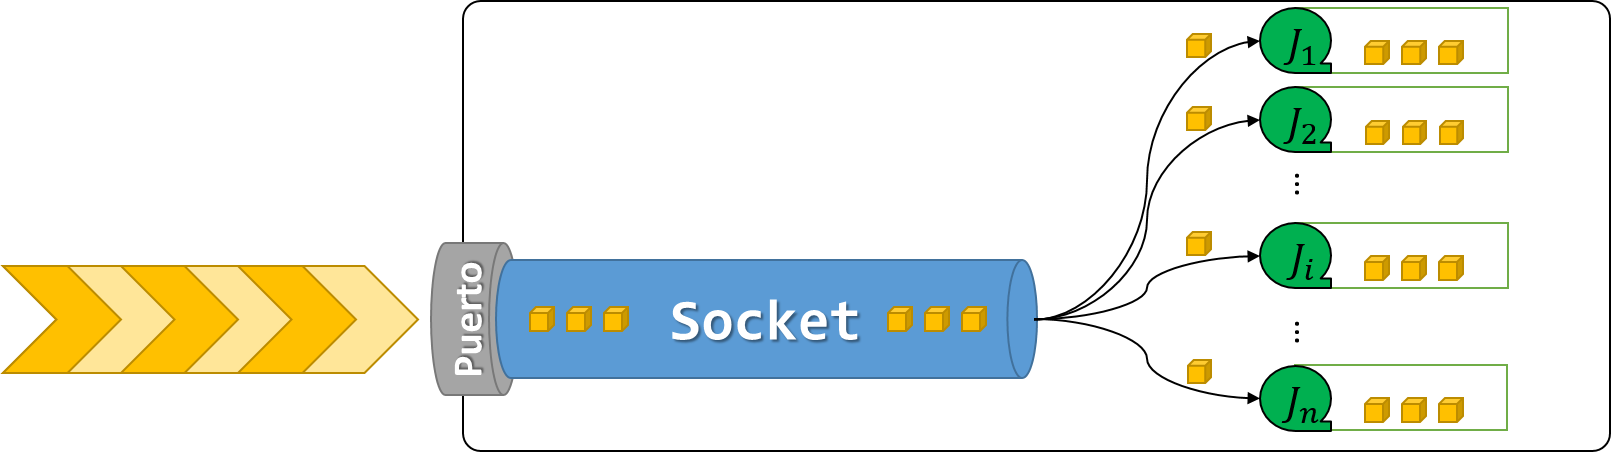
\includegraphics[scale=0.5]{imagenes/casoDeEstudio.png}
	\caption{Diagrama del \textbf{caso de estudio} que ilustra el diseño de la prueba de consumo de datos a través de un socket UDP usando múltiples hilos de ejecución.}
	\label{fig:testUDP}
\end{figure}

\subsubsection{Validación en Distintas Arquitecturas}

El comportamiento no escalable al usar threads es una característica que podría ser propia sólo de un tipo de arquitectura de recursos de hardware. Para comprobar el real alcance del problema antes descrito se evaluó la prueba de desempeño UDP en 3 escenarios de hardware diferente. Los tres escenarios de hardware se describen a continuación:

\begin{description}
\item[Laptop Quad Core] Laptop doméstico. Equipado con una CPU Intel(R) Core(TM) i5-5200U CPU @ 2.20GHz con tecnología \emph{hyperthreading} de Intel(R) y 6 GB de memoria. Un esquemático del sistema disponible en la figura \ref{fig:pc2}.
\item[PC Dual Socket] Computador de escritorio. Equipado con dos CPU Intel(R) Xeon(TM) CPU @ 2.80GHz, cada uno con tecnología \emph{hyperthreading} de Intel(R) y 2 GB de memoria interna. Imagen ilustrativa disponible en la figura \ref{fig:pc3}.
\item[Servidor 24 Cores] Equipo servidor multiprocesador. Equipado con dos CPU Intel(R) Xeon(R) CPU X5660 @ 2.80GHz, cada uno con tecnología \emph{hyperthreading} de Intel(R) y 24 GB de memoria, distribuidos en dos nodos NUMA de procesamiento, organizado en base a la \emph{Intel QuickPath Architecture}. Diagrama del sistema en imagen \ref{fig:pc1}.
\end{description}

\begin{figure}[h!]
	\centering
	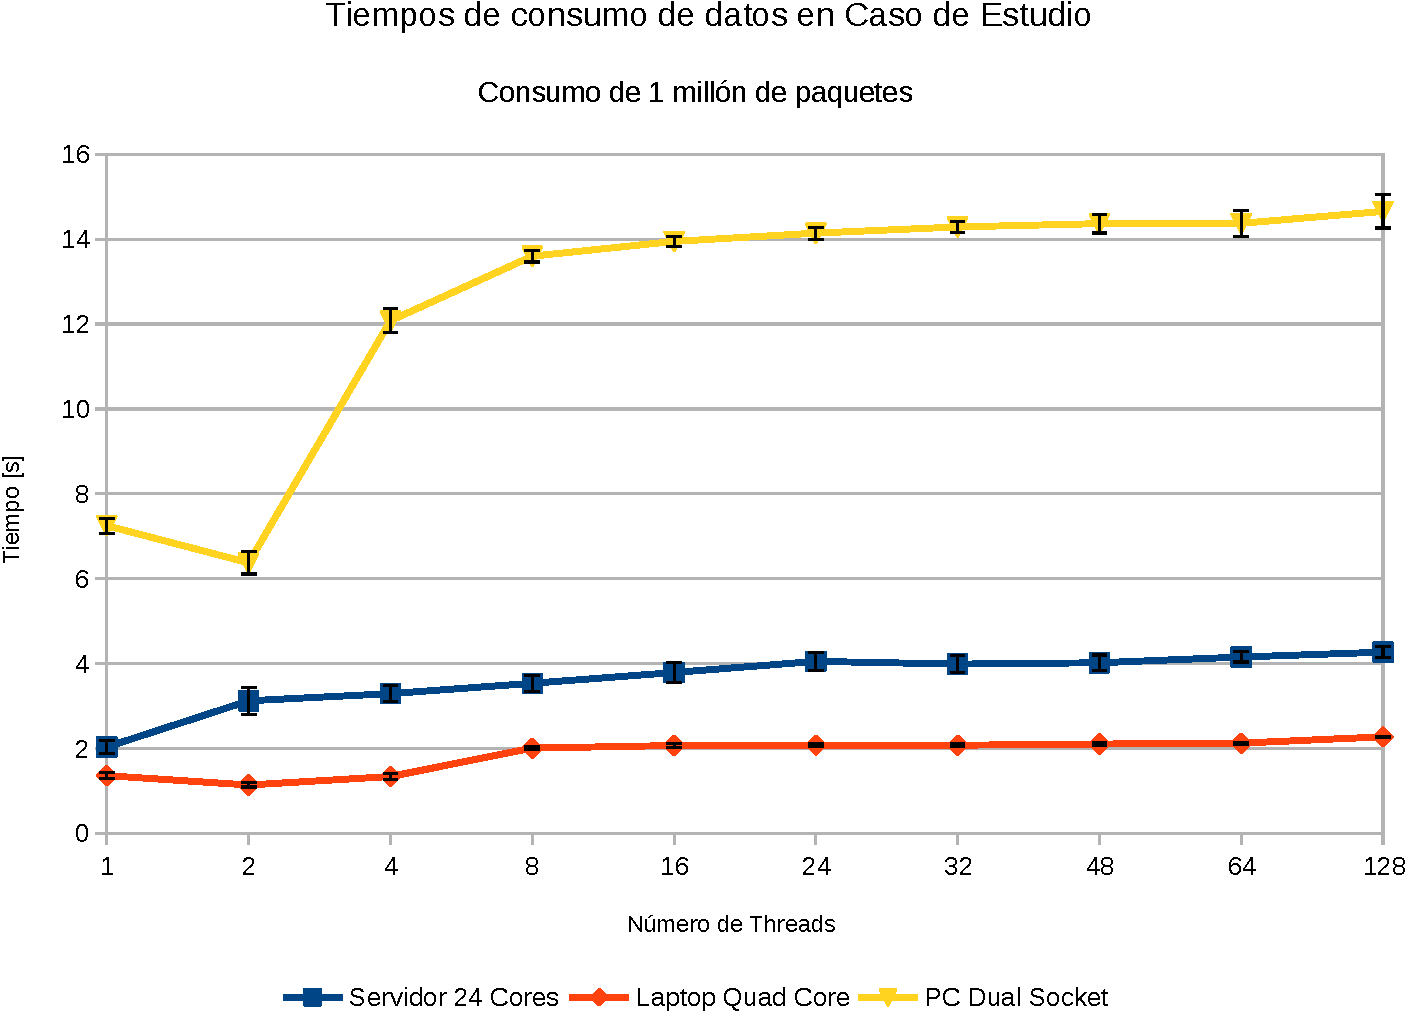
\includegraphics[scale=0.5]{resultados/transferenciaUDP1-crop.pdf}
	\caption{Grafico comparativo del rendimiento de prueba UDP entre distintas arquitecturas de hardware. Los valores mostrados son representativos de 60 repeticiones de la prueba de transferencia UDP.}
	\label{fig:tests_arch}
\end{figure}

\begin{figure}
\centering
\hspace*{\fill}
\subfigure[Pc2]{
	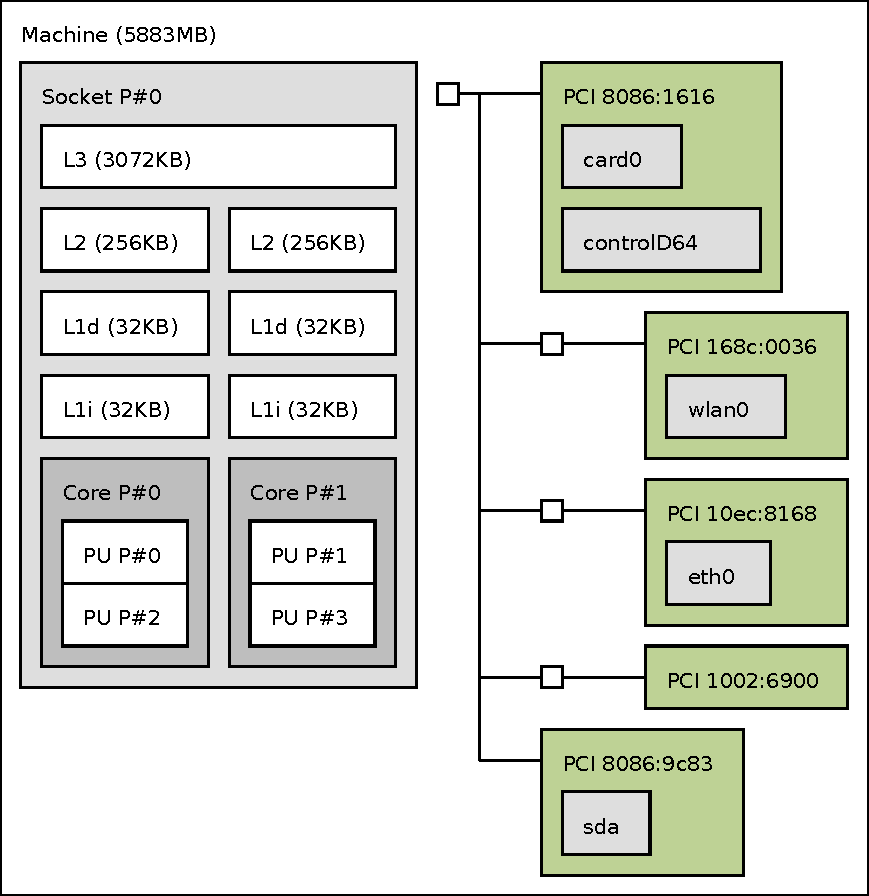
\includegraphics[height=.4\textwidth]{imagenes/pc2.pdf}
	\label{fig:pc2}
}\hspace*{\fill}
\subfigure[Pc3]{
	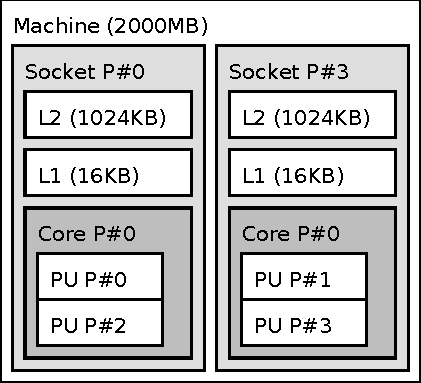
\includegraphics[height=.4\textwidth]{imagenes/pc3.pdf}
	\label{fig:pc3}
}
\hspace*{\fill}
\\
\subfigure[Pc1]{
	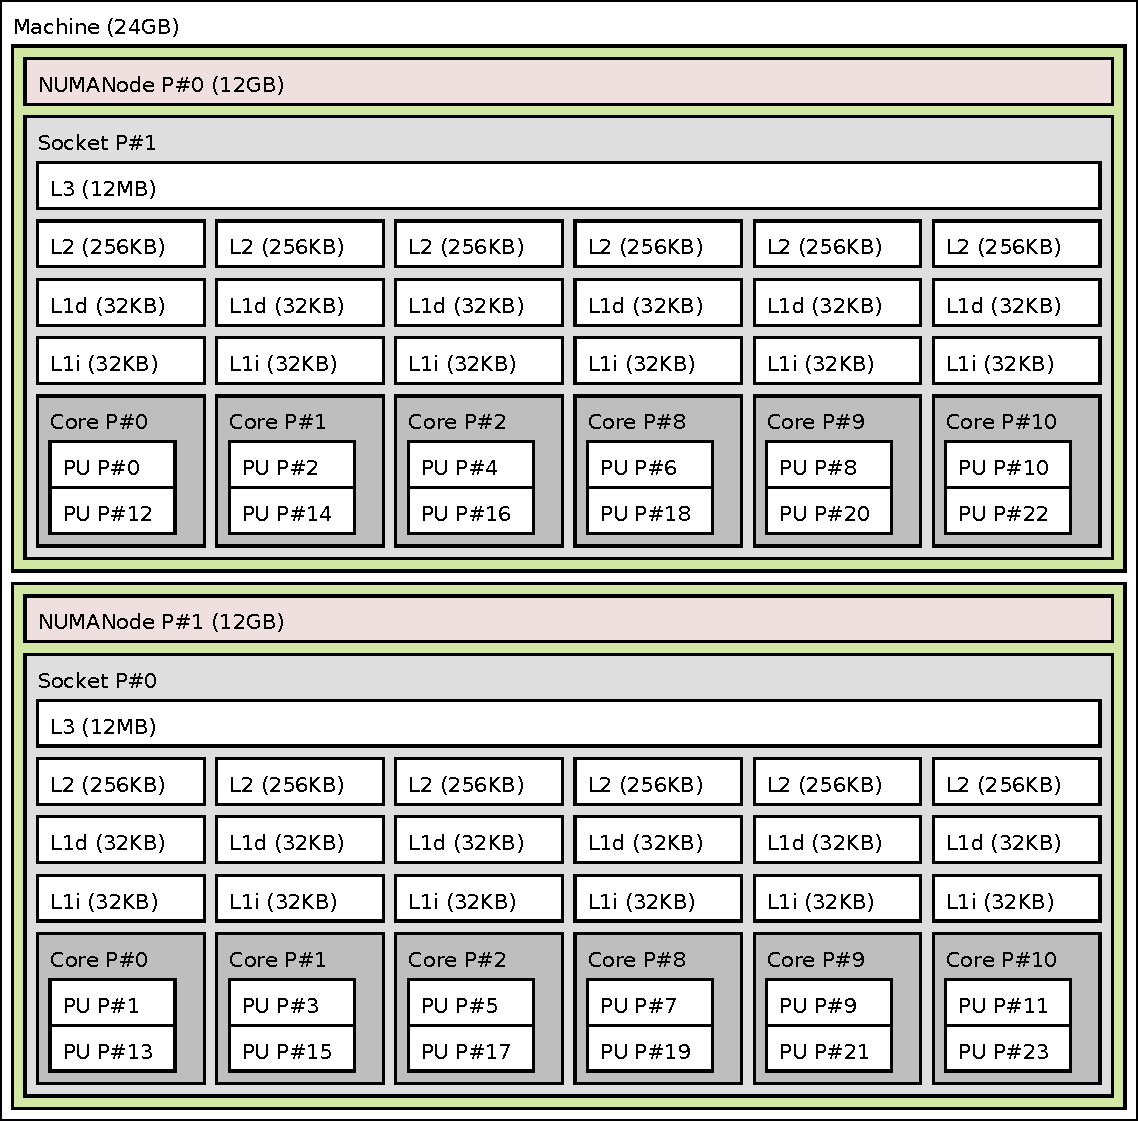
\includegraphics[width=.85\textwidth]{imagenes/pc1.pdf}
	\label{fig:pc1}
}
\caption{Esquemas de hardware de los 3 equipos evaluados para la validación del problema. Imágenes generadas con la herramienta \texttt{lstopo} del paquete \texttt{hwloc}.}
\end{figure}

De los resultados experimentales de la figura \ref{fig:tests_arch} se pueden rescatar dos aspectos relevantes:
\begin{itemize}
\item El primero, que el efecto de consumo concurrente es distinto entre los 3 escenarios estudiados, dejando en evidencia que las diferentes configuraciones de hardware en cada caso entregan diferente desempeño a la hora de aprovechar ejecuciones paralelas y de enfrentar escenarios de concurrencia.
\item El segundo, que el caso de mayor interés, ilustrado en la arquitectura del servidor multiprocesador presenta una situación de baja de desempeño a medida que se congestiona (o satura) más fuertemente el consumo de la interfaz de red, representada por el socket UDP. La tendencia es similar a la reportada por estudios anteriores que cuestionan la aplicabilidad de técnicas de paralelísmo en éste tipo de arquitecturas por no demostrar un mejor desempeño evidente \cite{post:facebook, paper:toshiba, tesis:diegoDCC}.
\end{itemize}

\begin{figure}[h!]
	\centering
	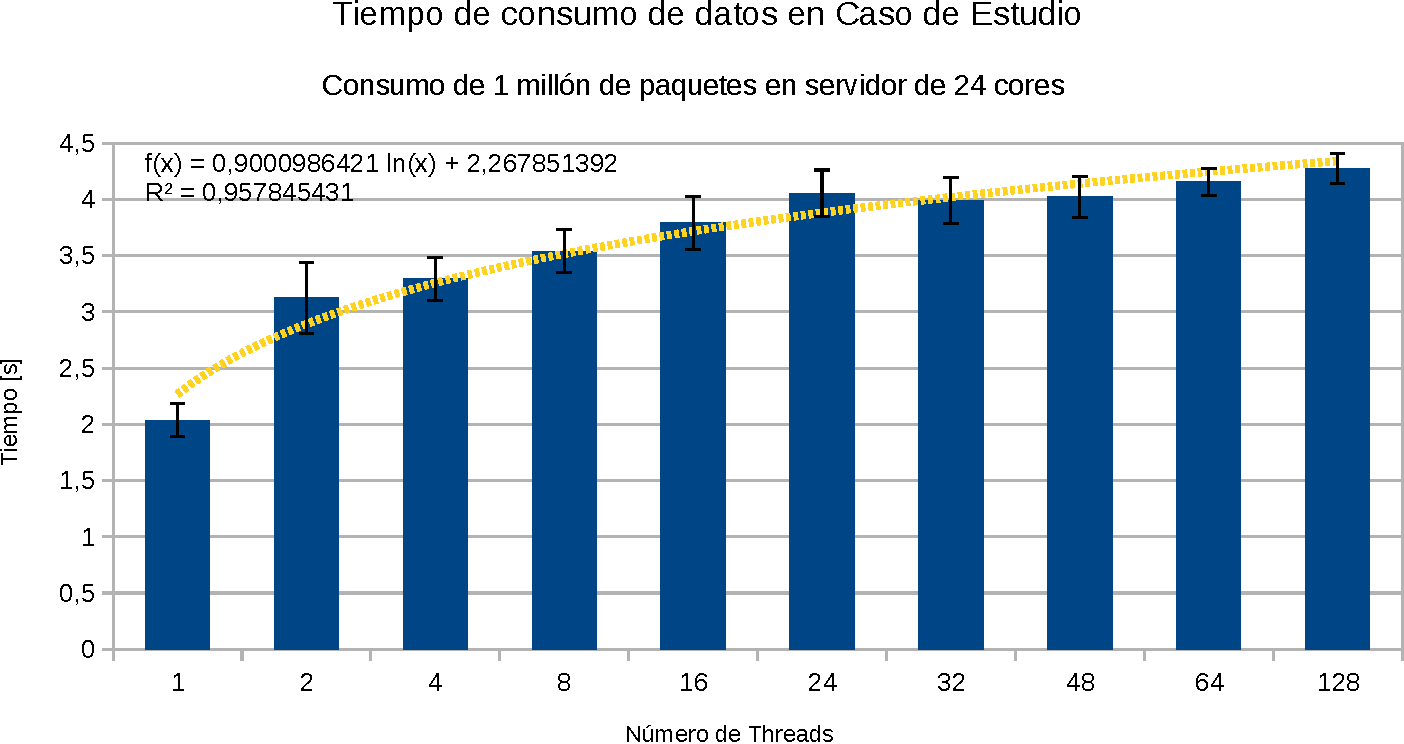
\includegraphics[scale=0.5]{resultados/transferenciaUDP2-crop.pdf}
	\caption{ZOOM.}
	\label{fig:tests_arch}
\end{figure}

Las conclusiones preliminares del estudio, apoyan la idea de continuar indagando la operación del caso de estudio en la arquitectura del servidor multiprocesador, que viene siendo el escenario típico para la operación DNS, que es el caso que nos inspira en ésta investigación.

\subsubsection{Validación en Distintas Versiones de Kernel de Linux}

Al igual que con la arista de hardware, el fenómeno de mal rendimiento de threads detectado podría ser propio de la componente de software del sistema, entendido como una determinada versión del kernel de Linux. Una sospecha que se acentúa al recordar que parte importante del código fuente del núcleo es heredado entre versiones y que las versiones más populares del kernel abarcan una importante razón de tiempo entre sus publicaciones. A continuación se muestra una línea de tiempo con algunas de las publicaciones más importantes del kernel de linux\footnote{\url{https://www.kernel.org/category/releases.html}}.


\definecolor{myhighlight}{RGB}{250,250,60}
\begin{center}
\scalebox{1.2}{
\begin{tabular}{r |@{\timeline} l}
3 Diciembre 2009 & 2.6.32\\
4 Enero 2012 & \colorbox{myhighlight}{3.2}\\
20 Mayo 2012 & 3.4\\
30 Junio 2013 & \colorbox{myhighlight}{3.10}\\
2 Noviembre 2013 & \colorbox{myhighlight}{3.12}\\
30 Marzo 2014 & \colorbox{myhighlight}{3.14}\\
7 Diciembre 2014 & 3.18\\
12 Abril 2015 & \colorbox{myhighlight}{4.0.4}\\
\end{tabular}
}
\end{center}

Las versiones destacadas son aquellas que se consideraron como entornos de estudio interesantes para la validación del problema. La justificación de ésta elección se basa en dos criterios: Primero, que el conjunto de versiones elegidas son todas \emph{Longterm Support} por lo que son la base principal en las ramas de desarrollo aledañas de otras versiones del kernel (sólo con correcciones de bugs importantes) y por lo tanto, son representativas de sistemas Linux más estables. Segundo, pues existen trabajos previos que ya se encargan de analizar el comportamiento estudiado en ediciones más antiguas del Kernel cómo en la versión base 2.6 \cite{tesis:diegoDCC}.

\begin{figure}[h!]
	\centering
	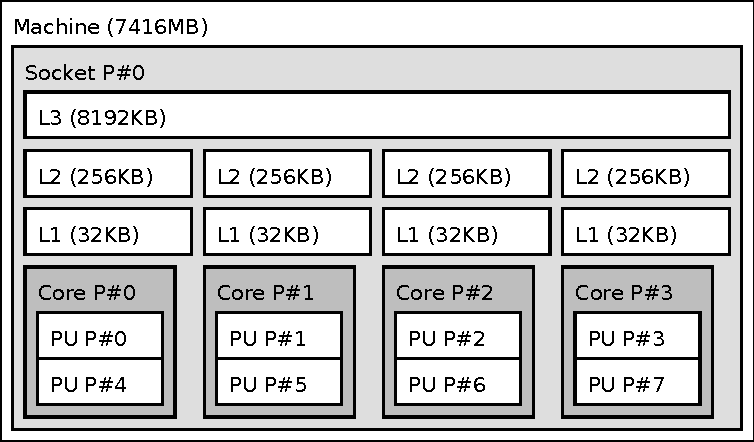
\includegraphics[scale=0.65]{imagenes/desktopkernelpc.pdf}
	\caption{Esquema de hardware del equipo donde se evaluó el rendimiento del caso de estudio sobre distintas versiones del kernel de Linux. El equipo corresponde a se compone de una CPU Intel(R) Core(TM) i7-4790 CPU @ 3.60GHz con tecnología \emph{hyperthreading} de Intel(R) y 8 GB de memoria.}
	\label{fig:desktop_kernel_pc}
\end{figure}

Para la evaluación, se instalaron las versiones destacadas de la línea de tiempo previamente mostrada en un equipo de prueba (Ver figura \ref{fig:desktop_kernel_pc}) en el cual se evaluó el caso de estudio ya propuesto, registrándose los distintos tiempos finales entre cada versión del kernel. Más allá de mostrar un incremento o reducción de tiempos con respecto a la arquitectura ilustrada en la máquina servidor multicore, el objetivo de ésta prueba busca evidenciar si existe una tendencia constante en el tiempo de la prueba entre las diferentes versiones del kernel. Un resultado comparativo de los distintos rendimientos entre versiones del kernel está ilustrado en la figura \ref{fig:tests_kernel}.


\begin{figure}[h!]
	\centering
	\hspace*{\fill}
	\subfigure[]{
		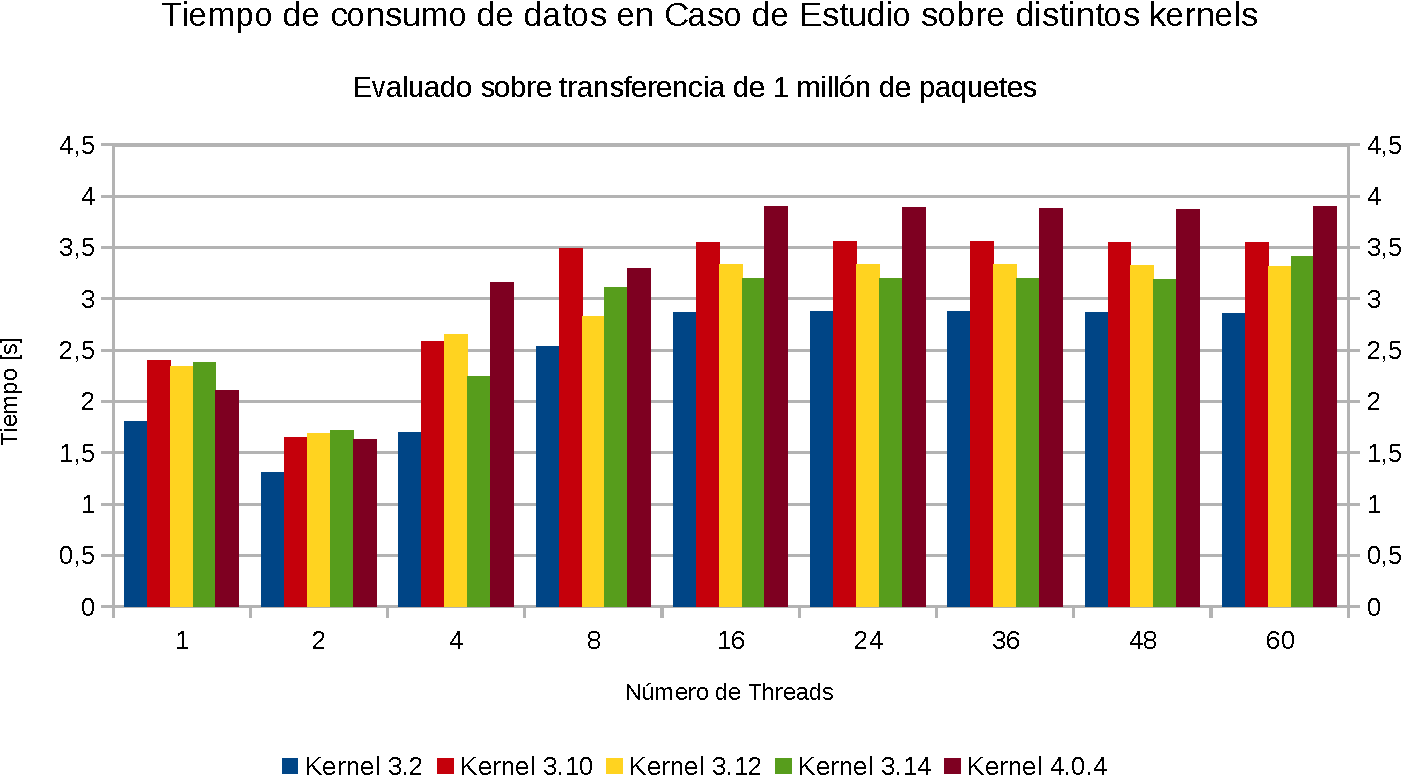
\includegraphics[width=.47\textwidth]{resultados/kernel1-crop.pdf}
		\label{fig:tests_kernel1}
	}\hfill
	\subfigure[]{
		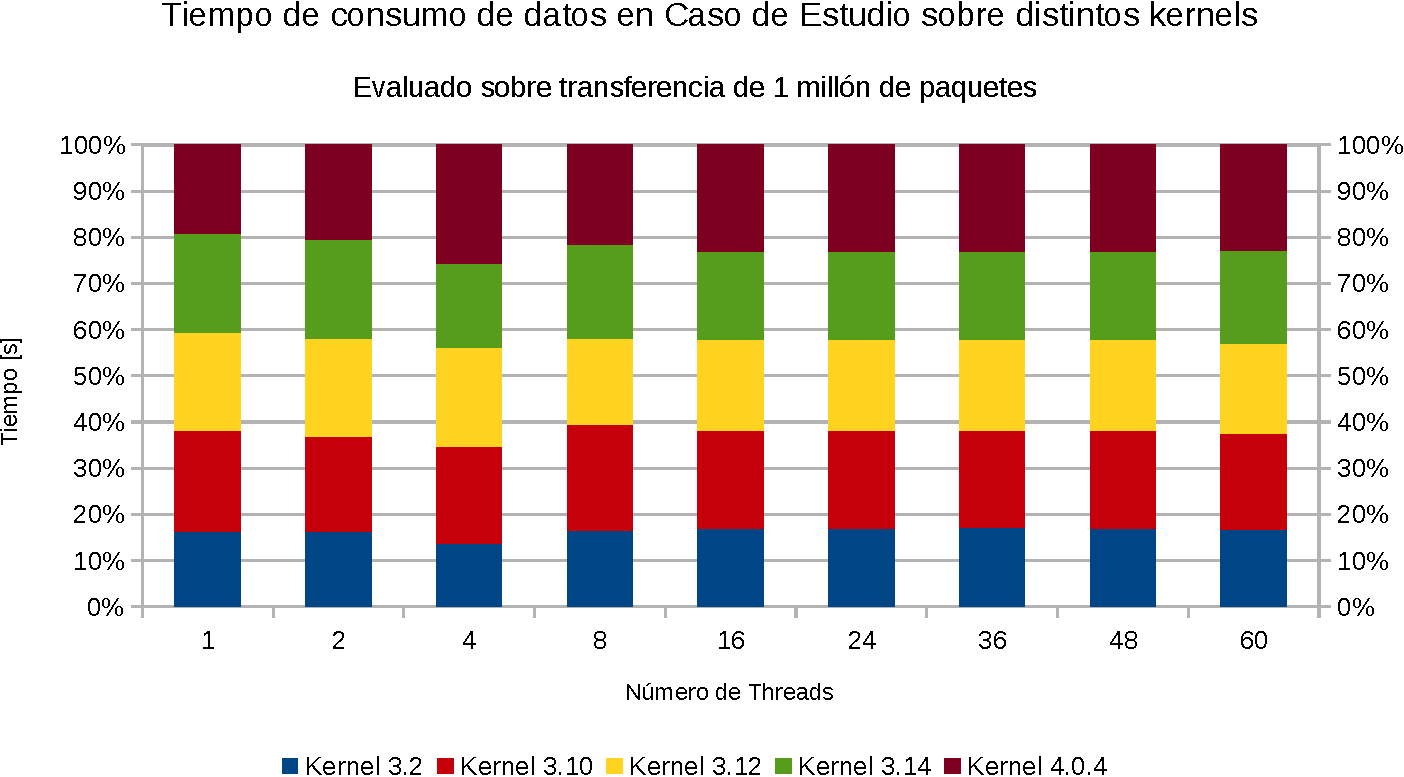
\includegraphics[width=.47\textwidth]{resultados/kernel2-crop.pdf}
		\label{fig:tests_kernel2}
	}
	\caption{Graficos comparativos del rendimiento de prueba UDP entre distintas versiones del Kernel. Los valores mostrados son representativos de 60 repeticiones de la prueba de transferencia UDP.}
	\label{fig:tests_kernel}
	\hspace*{\fill}
\end{figure}

Los resultados de esta prueba ilustran en primera instancia que las distintas versiones del kernel presentan distinto rendimiento sobre el caso de prueba estudiado, ello de acuerdo a los resultados del gráfico \ref{fig:tests_kernel1} dónde puede ser muy significativa la diferencia al incorporar threads en el consumo de datos. Sin embargo, de acuerdo con el gráfico \ref{fig:tests_kernel2}, donde se muestran las porciones de tiempo correspondientes al consumo de datos del socket cada configuración de hilos con respecto al tiempo total, se aprecian prácticamente comportamientos idénticos entre configuraciones independiente del kernel usado. Esta situación da a entender que, a pesar de que los tiempos sean diferentes entre versiones, las tendencias y comportamientos son uniformes entre las distintas versiones del kernel, por lo que la varianza de tiempos entre distintas versiones del kernel sería un fenómeno producido por ciertas optimizaciones o degradaciones del rendimiento en componentes que no son inherentes únicamente a nuestro caso de estudio.


Los resultados anteriores terminan por validar la persistencia del problema, descartando la responsabilidad del mismo a una única edición del kernel de Linux, y validando también la persistencia del problema mismo en arquitecturas de interés como lo son máquinas servidores multicore.

\subsection{Hipótesis del Problema}
Las sospechas iniciales del responsable de éste problema apuntan a un defecto que se esconda a nivel del núcleo del sistema operativo \cite{paper:toshiba,post:facebook}. Como ya se mencionó, desde su versión 2.6 el kernel de Linux incorporó capacidad de procesamiento simétrico multiprocesador (\emph{Symmetric Multi-Processing - SMP}), con esto el scheduler de tareas transfirió los hilos de ejecución paralelos al mismo núcleo del sistema, con el costo de tener que implementar protección para áreas completas de código y estructuras a fin de evitar modificaciones concurrentes. Para ello, Linux provee diversas primitivas de sincronización mencionadas en secciones anteriores a disposición de los programadores. Sin embargo, el módulo de redes del kernel de Linux data de versiones previas a la 2.6 que suponían entre sus recursos a monoprocesadores y que, por lo tanto, no consideraban operaciones simultáneas con múltiples procesadores como se consiguió con \emph{SMP}.

La sospecha inicial apunta a que probablemente, el efecto encontrado al evaluar diseños como el de la ilustración \ref{fig:multi_thread} es precisamente reflejo de un problema a nivel del kernel, donde alguna estructura de sincronización de bajo nivel está presentando un problema de contención que se traduce en una serialización de acceso, o similar, y que repercute en tiempos muertos en casos de concurrencia. Una sospecha que es avalada por los resultados obtenidos hasta éste punto de la investigación.

Tras importantes trabajos relacionados a nuestro caso de estudio, realizados por de líderes en la industria como Google  \cite{slides:googleReuseport}, se ha llegado a establecer una colección de hipótesis consensuadas de que son varios los factores que contribuyen a la degradación generalizada que se presenta. En Primer lugar, se postula un \textbf{punto de contención} generado a raíz de la compartición de la estructura socket entre varios hilos de ejecución, estructura que no estaría apropiadamente diseñada para sobrellevar un escenario de concurrencia como al que se expone en éste caso. Otra teoría para explicar ésta situación se basa en el fenómeno de los \textbf{rebotes de caché}, propios de un esquema \emph{SMP} pero que se vería acrecentado en situaciones como las descritas por la necesidad de mantener información estructural de los sockets entre varios hilos que se distribuirían entre los múltiples núcleos de procesamiento disponible. Una tercera línea apunta en atribuir las responsabilidades del mal desempeño a los \textbf{mecanísmos de distribución de tareas} (El denominado schedulling para escenarios de distribución de carga) del sistema operativo, el cual en entornos \emph{SMP} jugaría en contra, degradando el rendimiento al modificar la propiedad de localidad de los datos para con los procesos constantemente, ello por medio de migraciones de los procesos entre las CPU disponibles. Otra hipótesis hace referencia a la posibilidad de que sean los propios \textbf{canales de comunicación} los que presentan un bajo rendimiento en situaciones de concurrencia como la descrita y cuyo overhead terminaría impactando en los tiempos netos, entre otros.

El problema real es que ninguna de las distintas hipótesis previamente repasadas ha sido experimentalmente estudiada, con lo que no se ha podido validar ni refutar la veracidad de las mismas. No tener claridad sobre cuál es la componente responsable incurre en otros problemas como el no poder postular una solución que consiga solucionar correctamente el mismo, al no tener claro cuál arista trabajar. En los capítulos siguientes se postula encapsular las hipótesis antes planteadas en líneas de investigación para corroborar experimentalmente la validez de las mismas, para posteriormente, con un entendimiento mejorado del problema, postular un mecanismo alterno que permita aprovechar la capacidad multiprocesador para lograr mejores tiempos netos en el caso de estudio ilustrado.
